\section{PSP个体软件过程}

\begin{figure}[H]
    \vspace{-0.5em}
	\centering
	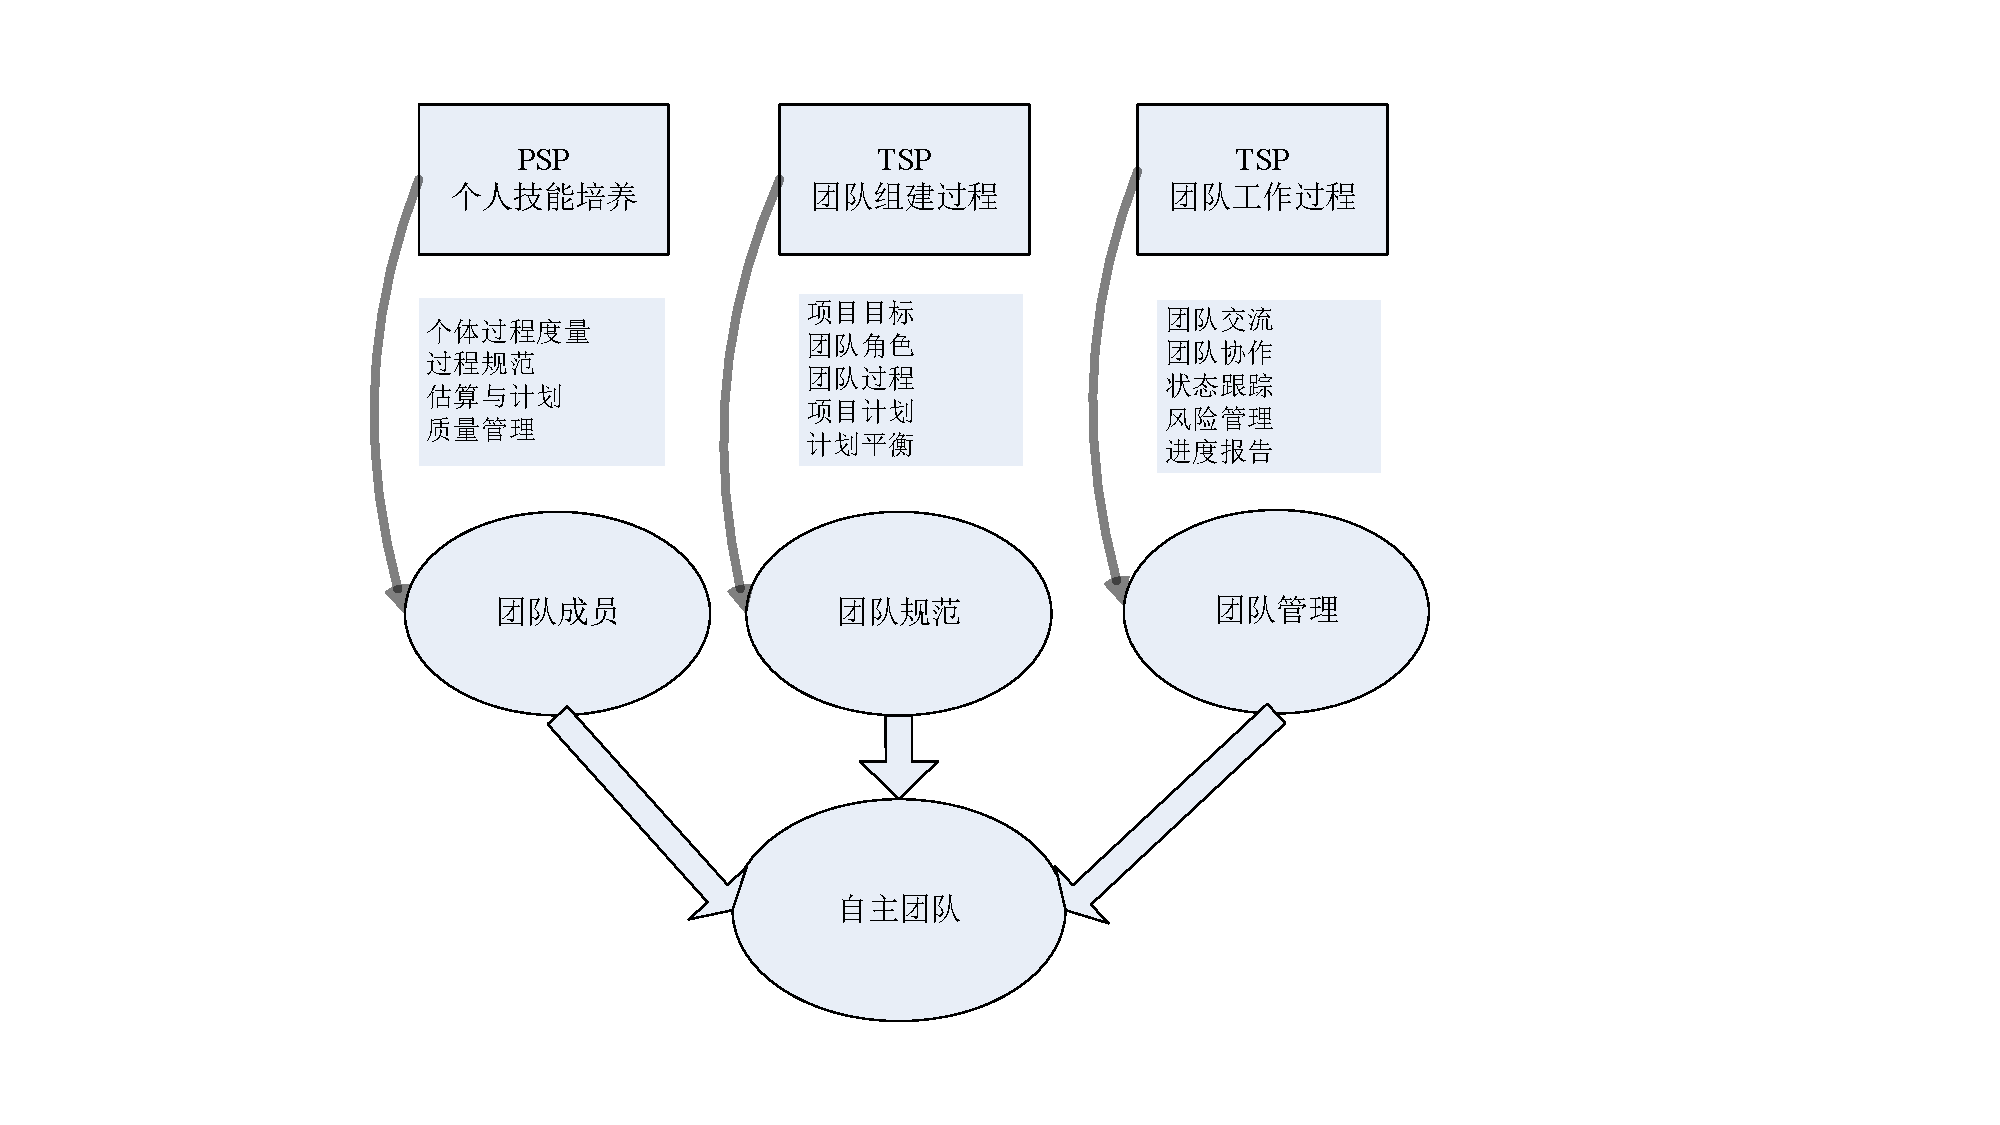
\includegraphics[width=0.7\textwidth]{images/PSP.pdf}
    \vspace{-1em}
\end{figure}

\subsection{PSP简介}
PSP是包括了数据记录表格、过程操作指南和规程在内的结构化框架

PSP着重于软件开发人员的个人能力提升,体现在估算能力、计划能力、计划执行以及质量管理等方面

基本的PSP包括策划、设计、编码、编译、单元测试以及总结等阶段
\begin{itemize}
    \item 每个阶段,都有相应的过程操作指南,用来指导该阶段的开发活动。
    \item 所有的开发活动都需要记录相应的时间日志和缺陷日志
\end{itemize}

\begin{figure}[H]
    \vspace{-0.5em}
	\centering
	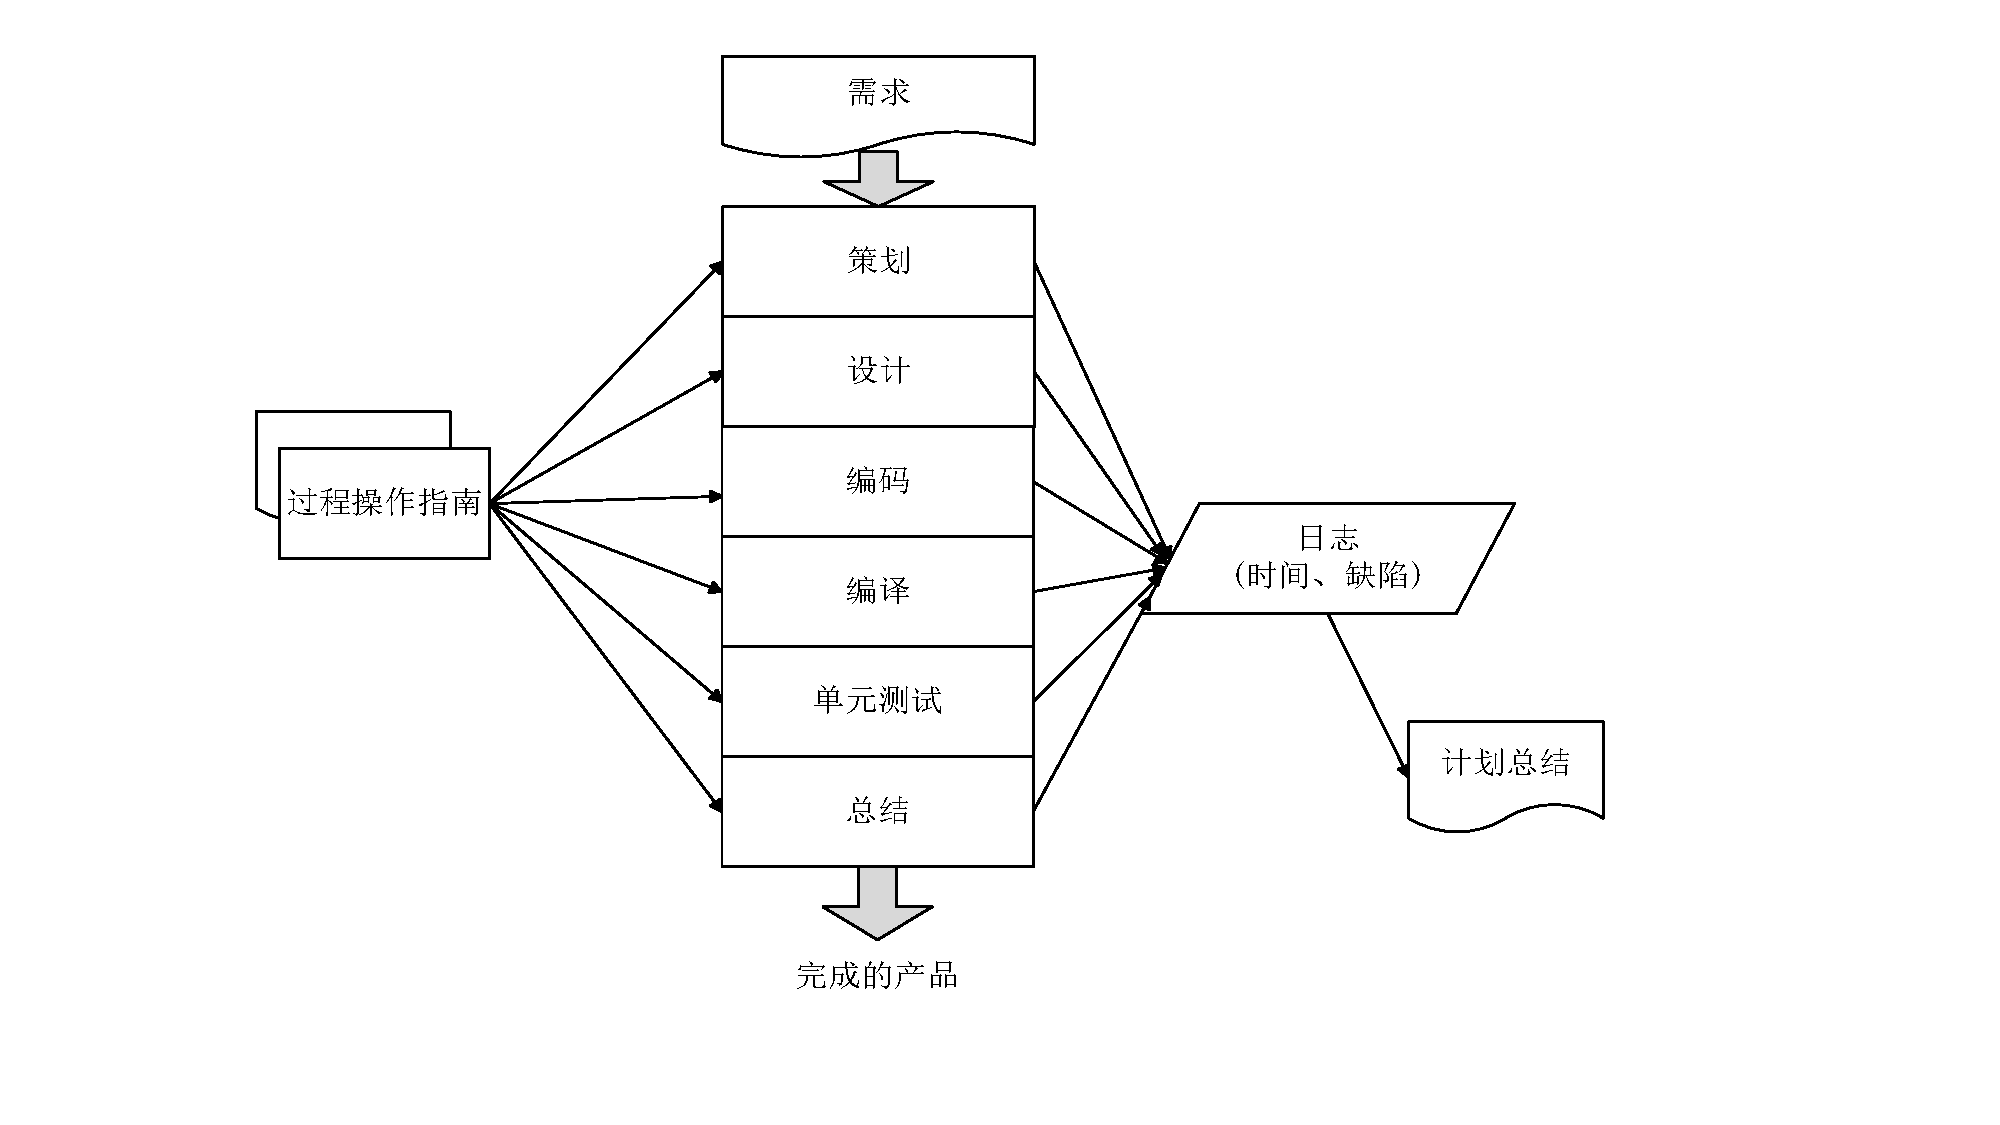
\includegraphics[width=0.7\textwidth]{images/PSP过程.pdf}
    \vspace{-1em}
\end{figure}

\subsubsection{PSP基本原理}
\begin{itemize}
    \item 软件系统的整体质量由该系统中质量最差的某些组件所决定
    \item 软件组件的质量取决于开发工程师所使用的开发过程
    \item 软件工程师应当自己度量、跟踪自己的工作流程,并建立持续的自我改进机制(在自己开发过程的偏差中学习、总结,并将这些经验教训整合到自己的开发实践),自己管理软件组件的质量
\end{itemize}
上述基本原理除了继续肯定“过程质量决定最终产品质量”这一软件过程改进的之外,更加突出了个体软件工程师在管理和改进自身过程中的能动性。这就形成了PSP的理论基础

\subsubsection{PSP的成熟度级别}
\begin{figure}[H]
    \vspace{-0.5em}
	\centering
	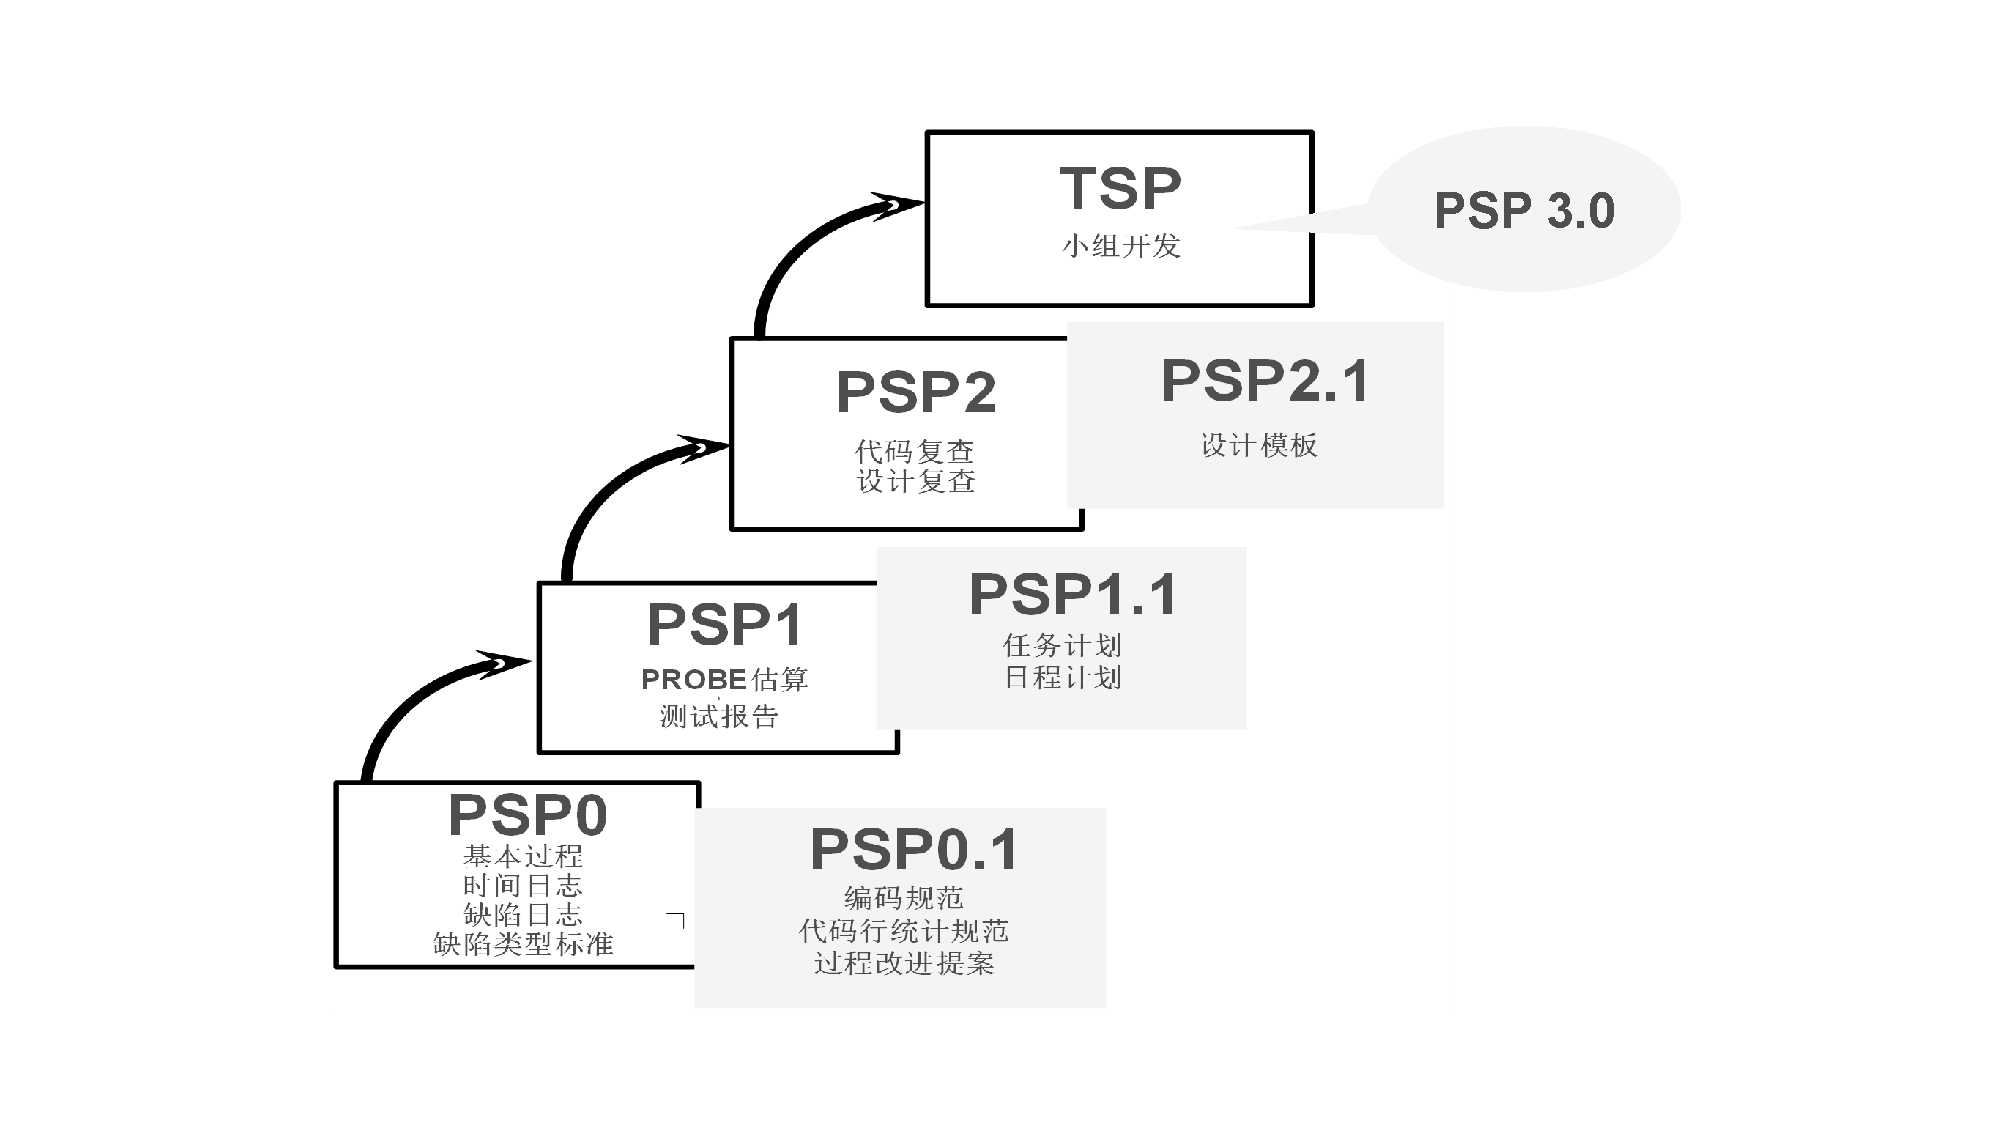
\includegraphics[width=0.6\textwidth]{images/PSP的不同级别.pdf}
    \vspace{-1em}
\end{figure}

\subsection{PSP的度量}

\subsubsection{基本度量项}
\begin{itemize}
    \item 度量时间:序号、所属阶段、开始时间、结束时间、中断时间、净时间、中断原因
    \item 度量缺陷:序号、发现日期、注入阶段、消除阶段、消除时间、关联缺陷、缺陷产生原因
    \item 度量规模:使用PROBE方法
    \vspace{-0.8em}
    \begin{multicols}{2}
        \begin{itemize}
            \item 选择的规模度量方式必须反映开发成本
            \item 度量规模必须被精确定义
            \item 度量规模必须有自动化方法统计
            \item 有助于早期规划
        \end{itemize}
    \end{multicols}
    \vspace{-1em}
    \item 日程(TSP)
\end{itemize}

\subsubsection{度量的作用}
\begin{itemize}
    \item 度量体现着决策者对试图要实现的目标的关切程度
    \item 度量帮助过程的实践者了解过程状态,理解过程偏差
\end{itemize}

\subsubsection{规模度量标准}
\vspace{-0.8em}
\begin{multicols}{2}
    \begin{enumerate}[label=\arabic*.]
        \item 选择的度量方式必须反映开发成本
        \item 选择的度量方式必须精确
        \item 选择的度量方式必须能用自动化方法来统计
        \item 选择的度量方式必须有助于早期规划
    \end{enumerate}
\end{multicols}
\vspace{-1em}

\subsubsection{规模的度量的困境}
精确的度量方式往往不便于早期规划;有助于早期规划的度量往往难以生成精确度量结果

\subsubsection{考试题目}
\begin{problem}
为什么精确的度量方式往往不便于早期规划,而有助于早期规划的度量往往难以产生精确度量结果?
\end{problem}

\begin{problem}
对比度量方式 LOC 和 FP
\vspace{-0.5em}
\begin{spacing}{1.2}
    \centering
    \begin{longtable}{|m{2.5cm}<{\centering}|m{5.5cm}|m{4.5cm}<{\centering}|m{1.7cm}|}
        \hline
        \multicolumn{2}{|c|}{LOC}                                                & \multicolumn{2}{c|}{FP}                               \\ \hline
        \multicolumn{1}{|c|}{LOC优点}                 & \multicolumn{1}{c|}{LOC缺点} & \multicolumn{1}{c|}{FP优点} & \multicolumn{1}{c|}{FP缺点} \\ \hline
        LOC是软件开发项目的生成品,容易进行计算
        & 
        \vspace{-1em}
        \begin{enumerate}[label=\arabic*.,leftmargin=1em]
            \item LOC测量依赖于程序设计语言,不同语言产生结果存在偏差
            \item 对代码量少但设计精巧的程序产生不利评判
            \item 不适合非过程语言
            \item 在软件项目开发前或开发初期估算代码行数非常困难
            \vspace{-1.3em}
        \end{enumerate}                           
        & 
        \vspace{-1em}
        \begin{enumerate}[label=\arabic*.,leftmargin=1em]
            \item 和程序设计语言无关
            \item 面向过程和非过程语言均适合
            \item 基于项目开发初期就可能得到的数据
            \vspace{-1.3em}
        \end{enumerate}    
        & 计算基于主观而非客观数据 \\ \hline
    \end{longtable}
	\end{spacing}
\vspace{-1em}
\end{problem}

\begin{problem}
解释过程度量项定义时应当注意的方面,并且据此评价PSP基本度量元的合理之处?
\end{problem}

\begin{problem}
如何对某个软件产品组件进行产品质量评价?可以选择哪些度量元,这些度量元如何辅助判断产品组件的质量?
\end{problem}

\subsection{PROBE方法}
估算的目的是给各类计划提供决策依据

\subsubsection{估算原理}
设置合理的代理作为\textbf{精确度量}和\textbf{早期规划}需要的度量之间的桥梁:相对大小矩阵。相对大小而非绝对大小

\subsubsection{PROBE方法引入}
估算房子面积大小
\vspace{-0.8em}
\begin{multicols}{2}
    \begin{itemize}
        \item 使用房间相对大小矩阵
        \item 使用房间作为代理
    \end{itemize}
\end{multicols}
\vspace{-1em}

\begin{figure}[H]
    \vspace{-0.5em}
	\centering
	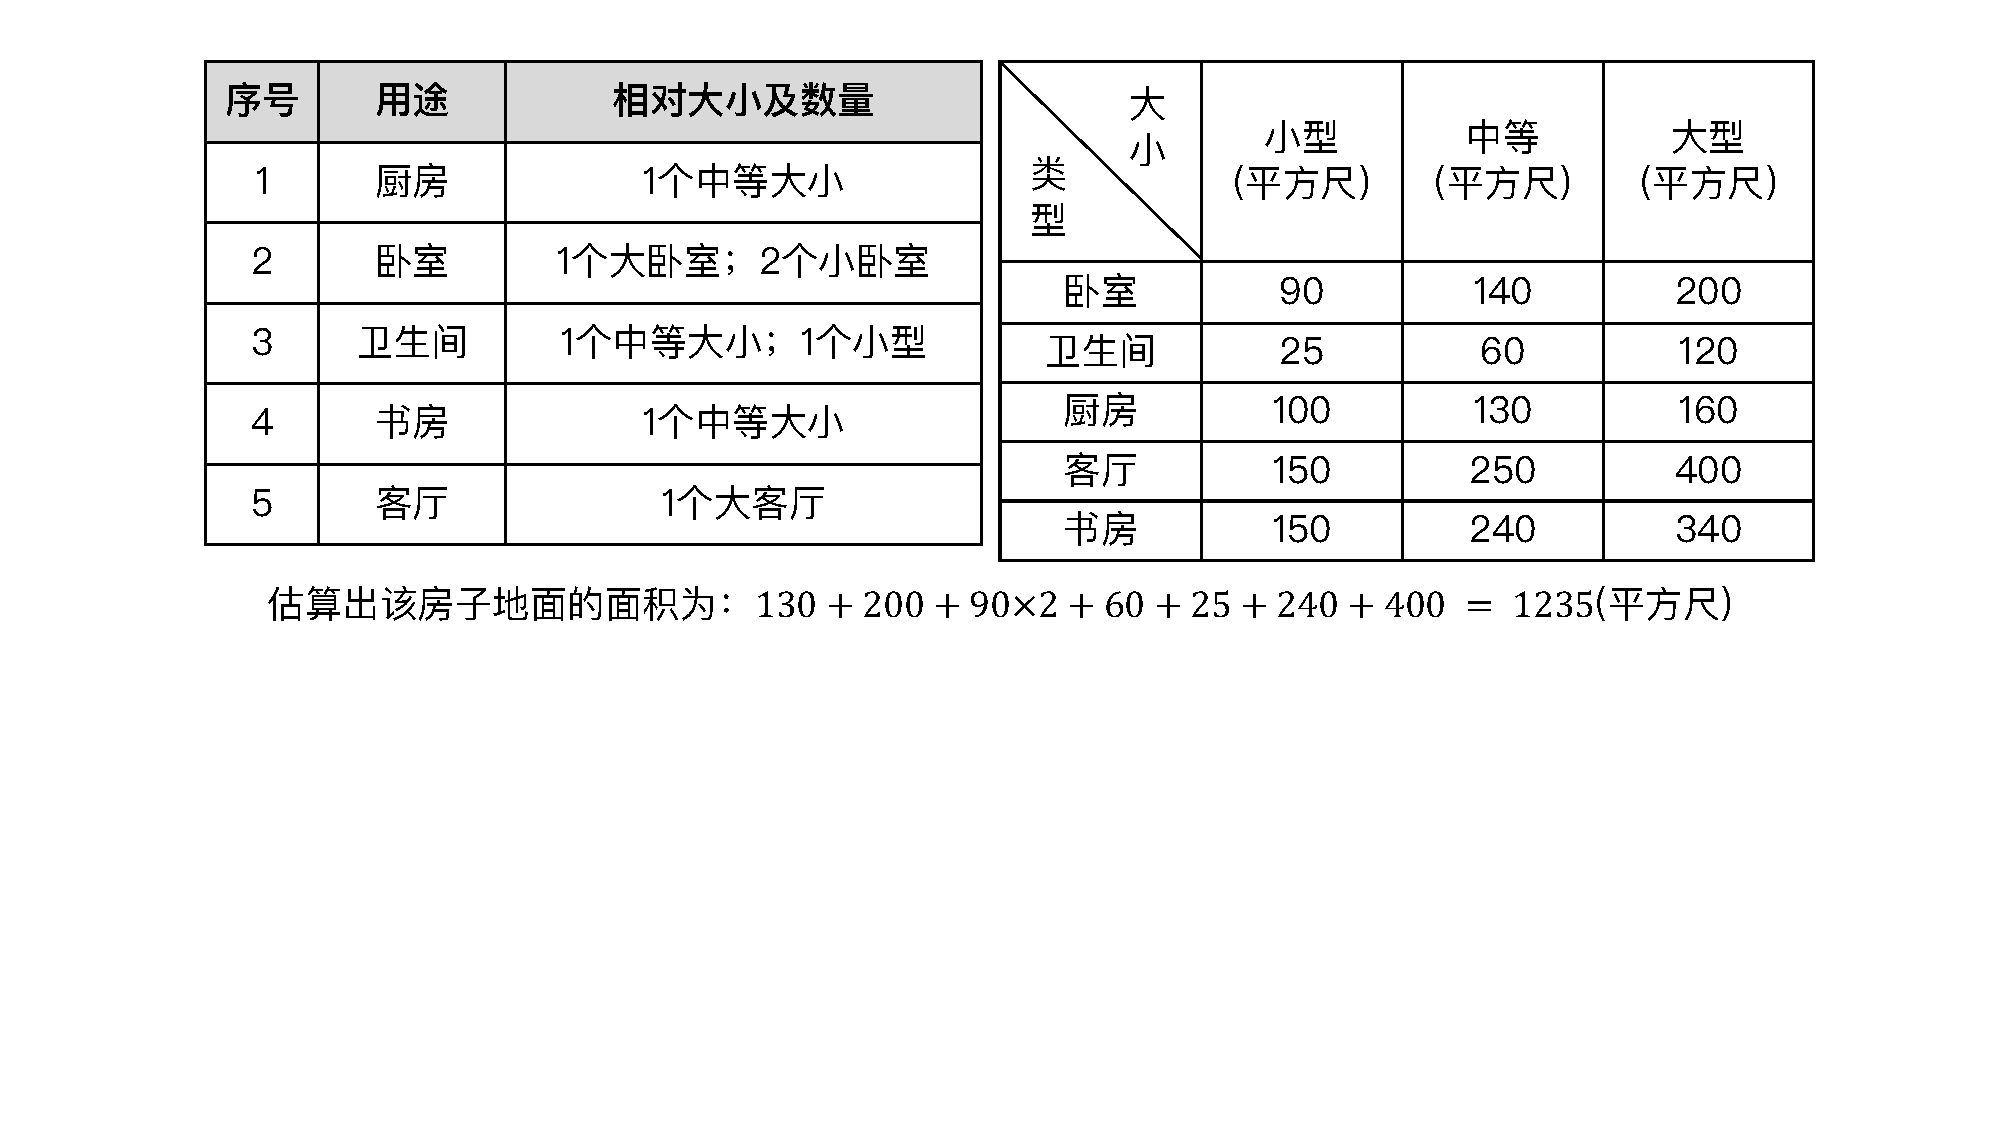
\includegraphics[width=0.95\textwidth]{images/PROBE方法例子.pdf}
    \vspace{-1em}
\end{figure}

\subsubsection{PROBE方法思想}
在PROBE估算中,需要建立自己的代码库,以跟踪所有程序的规模和工作量,而代码库中的每个组件都有设定的类型(计算、逻辑或数据等)和规模(非常小、小、中、大、非常大)
\begin{itemize}
    \item 如果新建立的组件与以前建立的组件类似,那么新组件所需的工作量与旧组件一样
    \item 当开始一个新项目时,我们可以将任务划分成与代码库中组件相似的类型和规模,然后利用线性回归方法来估算项目的工作量
\end{itemize}

估算本质上是一种猜测,追求的目标是一致性以及估算结果的使用者对估算结果的信心
\begin{itemize}
    \item PROBE方法通过定义估算过程和数据收集以及使用的框架,使得估算结果可以尽可能一致,从而使得一些统计方法可以用来调整估算结果,增强用户对估算结果的信心
    \item PROBE方法非常依赖高质量的历史数据,一旦数据不完整或缺失,会导致估算结果有明显偏差
\end{itemize}

\subsubsection{通用计划框架}
\begin{figure}[H]
    \vspace{-0.5em}
	\centering
	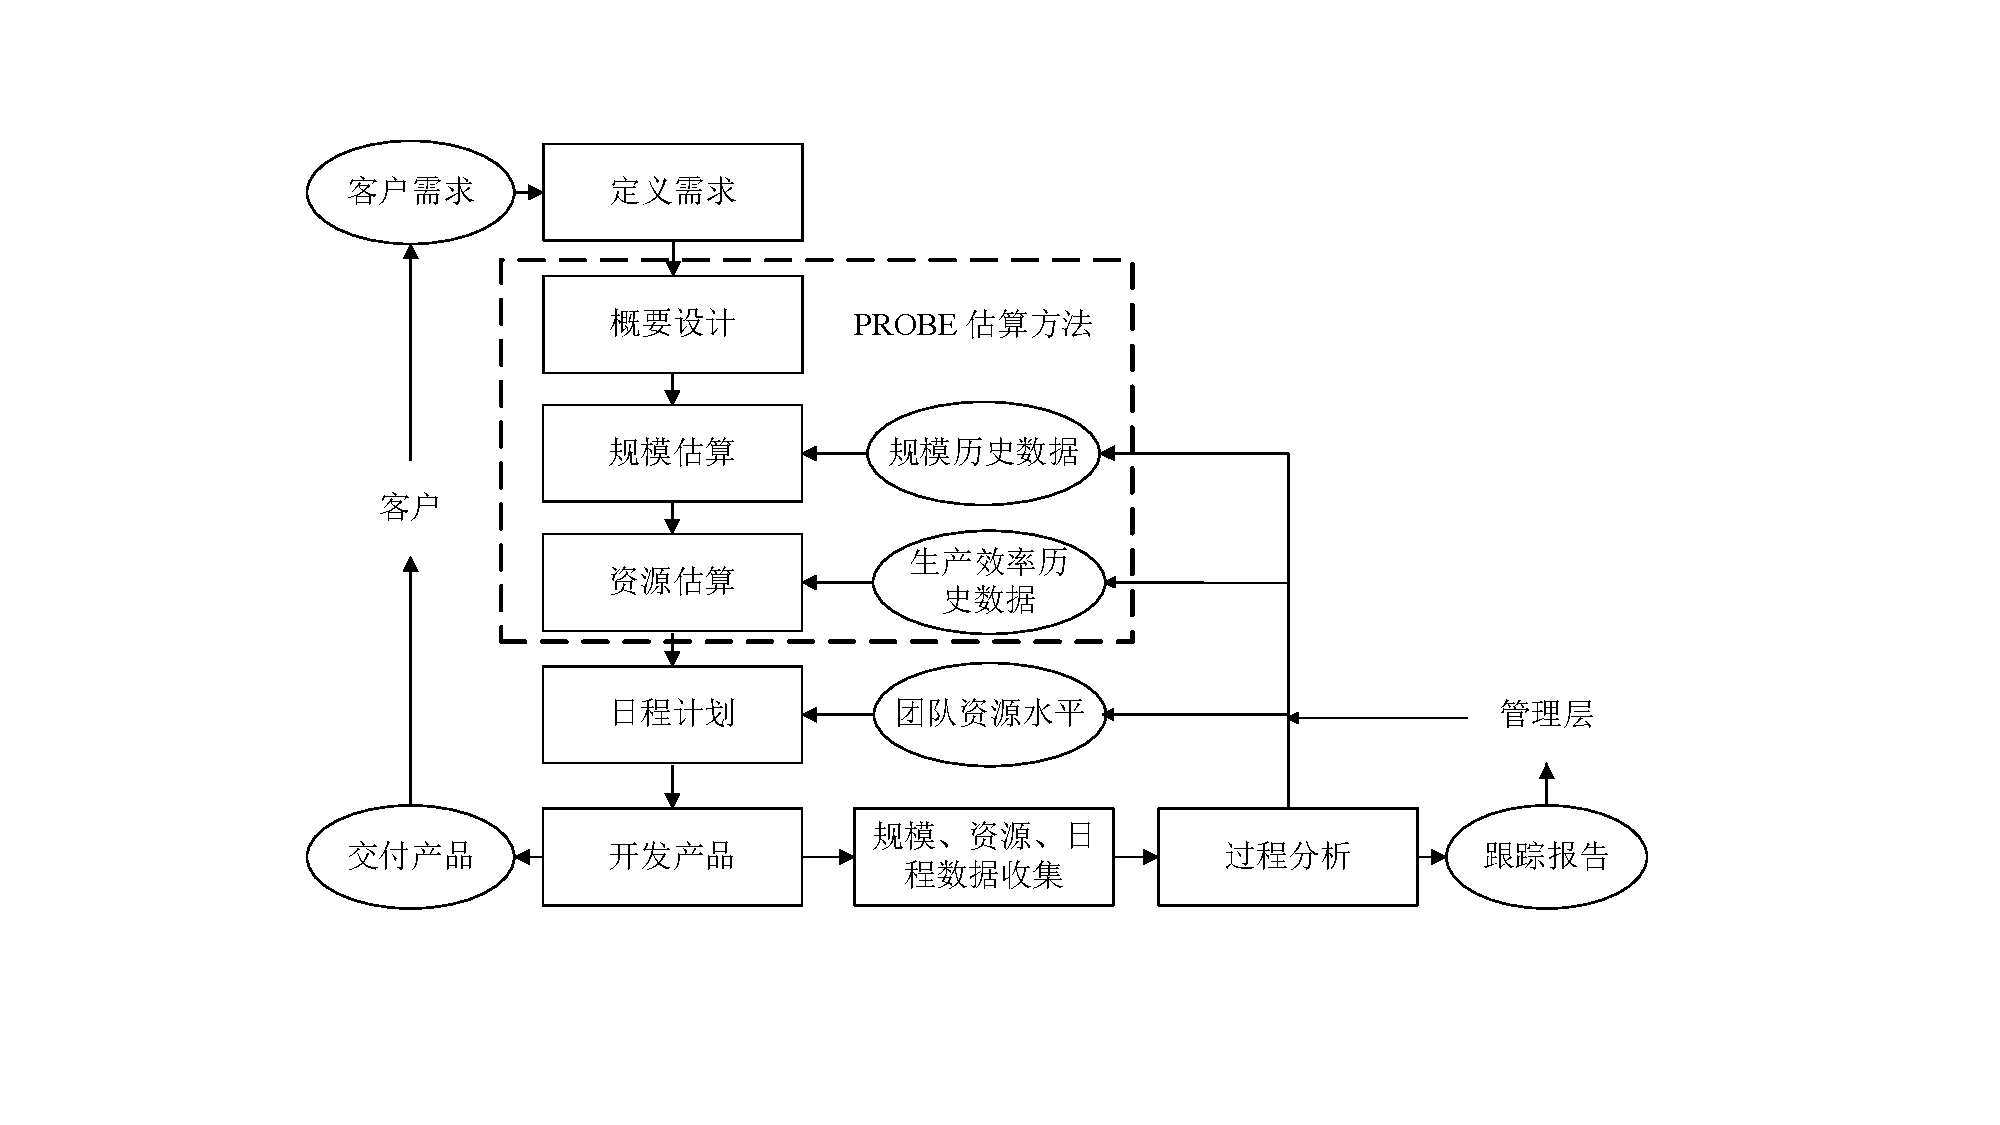
\includegraphics[width=0.75\textwidth]{images/通用计划框架.pdf}
    \vspace{-1em}
\end{figure}

上述框架中,哪些步骤必须人为的干预
\vspace{-0.8em}
\begin{multicols}{2}
    \begin{itemize}
        \item 定义需求
        \item 概要设计:划分由人为开始,规模划分好之后估算是自动产生的
        \item 日程计划
    \end{itemize}
\end{multicols}
\vspace{-1em}

这会带来什么的好处?比较容易扛住别人的质疑
\begin{itemize}
    \item 攻击点:资源和时间是否被高估了
    \item 解决:估算没有代码行,PROBE只有功能点是大中小
\end{itemize}

\begin{problem}
请简要描述按照通用计划框架,为了开发合理的项目计划,应该要做哪些估算?PROBE方法充当什么角色。

估算框架如上图,虚线框即为PROBE,用来完成规模和资源的评估
\end{problem}

\subsubsection{PROBE估算过程}
概要设计:
\vspace{-0.8em}
\begin{multicols}{2}
    \begin{enumerate}[label=\arabic*.]
        \item 确定产品功能,以及产生这些功能所需的程序组件/模块
        \item 将程序组件/模板与你之前写的程序相比较,估算它们的规模
        \item 最后将程序组件/模块估算综合给出总规模
    \end{enumerate}
\end{multicols}
\vspace{-1em}

估算要点:
\vspace{-0.8em}
\begin{multicols}{2}
    \begin{itemize}
        \item 尽可能划分详细一些:估算多个部件的时候,总的误差会比各个部件的误差的总和小
        \item 建立对结果的信心
        \item 依赖数据
        \item 估算要的是过程,而非结果,估算的过程是相关干系人达成一致共识的过程
    \end{itemize}
\end{multicols}
\vspace{-1em}

\paragraph{注意点1:整理历史数据}~{} \par
以估算规模为例,可以假定代理规模与实际程序规模之间存在简单关系映射、正态分布、对数正态分布,也可以假定不知道两者之间的关系,按照线性回归方法进行计算
\vspace{-0.5em}
\begin{spacing}{1.2}
    \centering
    \begin{longtable}{|m{1.5cm}<{\centering}|m{7cm}|m{6cm}|}
        \hline
        \textbf{方法} & \multicolumn{1}{c|}{\textbf{方法描述}} & \multicolumn{1}{c|}{\textbf{方法特点}} \\ \hline
        简单方法
        & 最小值作为$VS$,最大值作为$VL$,中值作为$M$,$VS$与$M$均值作为$S$,$VL$与$M$均值作为$L$
        & 优点:计算简单;缺点:不稳定 \\ \hline
        正态分布法
        & 均值作为$M$,计算标准差$\sigma$,则$S=M-\sigma$,$VS=M-2\sigma$,$L=M+\sigma$,$VL=M+2\sigma$
        & 优点:相对稳定,在历史数据基本符合正态分布的情况下,可以给出非常好的相对大小矩阵 \\ \hline
        对数正态分布法
        & \vspace{-1em}
        \begin{enumerate}[label=\arabic*.,leftmargin=1em]
            \item 以$e$为底计算所有数据的自然对数
            \item 取对数之后的值的均值作为$M$,计算相应标准差$\sigma$,$S=M-\sigma$,$VS=M-2\sigma$,$L=M+\sigma$,$VL=M+2\sigma$
            \item 取反对数
        \vspace{-1.3em}
        \end{enumerate}
        & 优点:更加符合人们对于程序的规模的直观感觉,因为大多数人习惯写很多规模很小的程序,少量规模较大的程序 \\ \hline
        线性回归方法
        & \vspace{-1em}
        \begin{enumerate}[label=\arabic*.,leftmargin=1em]
            \item 计算的时候计算了两组线性回归的参数,也就是项目所需的资源并不是直接由程序规模和历史数据中的生产效率相除得到。程序的复杂度和程序规之间并不是简单的正相关关系。
            \item 线性回归方法估算的是一定概率条件下估算值的分布。例如最终实际程序规模有90\%的可能性落在$(a, b)$区间内
            \item Range为在一定概率条件下的变化区间,而$p$为概率
            \item Variance为扰动程度:有时候,历史数据中的一些极端数据会造成相关性的“假象”,故需要先进行数据除噪
            \vspace{-1em}
            $$\begin{array}{l}
            Plan\ Size = \beta_{0\ size} + \beta_{1\ size}(E) \\
            Plan\ Time = \beta_{0\ time} + \beta_{1\ time}(E) \\
            Range = t(p,df)\delta\sqrt{1 + \frac{1}{n} + \frac{(x_k-x_{avg})^2}{\sum\limits_{i=1}\limits^{n}(x_i-x_{avg})^2}} \\
            Variance = \delta^2 = \frac{1}{n-2}\sum\limits_{i=1}\limits^n(y_i - \beta_0 - \beta_1x_i)^2 \\
            \end{array}$$\vspace{-1.8em}
        \vspace{-1.3em}
        \end{enumerate}
        & \vspace{-1em}
        \begin{enumerate}[label=\arabic*.,leftmargin=1em]
            \item Plan Size和估算的类数量不呈现45度,是受到了估算误差和方法外代码的数量共同影响
            \item 该方法没有使用生产效率进行计算,为什么在PROBE中不使用生产效率?这样子使用好不好?因为Plan Size是在一个范围内波动,生产效率也在一个范围内波动,如果将生产效率作为分母,那么可能会导致更大的误差,也就违背了误差的出发点
            \item 估算能力的强弱关注是多稳定,而不是多接近具体的实际情况
            \vspace{-1.3em}
        \end{enumerate} \\ \hline
    \end{longtable}
	\end{spacing}
\vspace{-1em}

\paragraph{注意点2:处理有限的历史数据}~{} \par
规模估算:
\begin{itemize}
    \item 往往可以依据历史数据来完成,使用代理规模与实际程序规模之间的关系。
    \item 其原因在于规模估算结果的偏差产生原因相对客观,偏差可以用以修正新的估算结果。
    \item 估算规模对历史数据的要求如下,其中$r$为相关性(两组数据之间相互关联的程度,PSP中要求$r\geq 0.7$),其中$S$为显著性(两组数据的相关关系出现的偶然性,PSP要求$s\leq 0.05$)
\end{itemize}

\vspace{-0.5em}
\begin{spacing}{1.2}
    \centering
    \begin{longtable}{|m{2.3cm}<{\centering}|m{3cm}|m{4cm}|m{2.3cm}<{\centering}|}
        \hline
        \textbf{PROBE方法} & \multicolumn{1}{c|}{\textbf{数据要求}} & \multicolumn{1}{c|}{\textbf{数据质量要求}}                                                 & \multicolumn{1}{c|}{\textbf{计算方法}} \\ \hline
        A & 3组或者3组以上代理规模(E)与实际程序规模 &
        \vspace{-1em}
        \begin{enumerate}[label=\arabic*.,leftmargin=1.2em,itemsep=-2pt]
            \item $r\geq 0.7$
            \item $s\leq 0.05$
            \item $\beta 0 \leq$ 估算结果的25\%
            \item $0.5\leq \beta 1 \leq 2$    
        \vspace{-1.3em}
        \end{enumerate}
        & 略 \\ \hline
        B & 3组或者3组以上计划程序规模与实际程序规模 &
        \vspace{-1em}
        \begin{enumerate}[label=\arabic*.,leftmargin=1.2em,itemsep=-2pt]
            \item $r\geq 0.7$
            \item $s\leq 0.05$
            \item $\beta 0 \leq$ 估算结果的25\%
            \item $0.5\leq \beta 1 \leq 2$    
        \vspace{-1.3em}
        \end{enumerate}
        & 略 \\ \hline
        C & 有历史数据 & 无 & 按比例调整 \\ \hline
        D & 没有历史数据 & 无 & 猜测 \\ \hline
    \end{longtable}
	\end{spacing}
\vspace{-1em}

时间估算:
\begin{itemize}
    \item 使用代理规模和实际开发时间的关系。
    \item 时间估算的偏差产生原因更加复杂:一方面和规模有关,另一方面和人的主观能动性有关
    \item 历史数据中的时间偏差可参考价值不大
\end{itemize}

\vspace{-0.5em}
\begin{spacing}{1.2}
    \centering
    \begin{longtable}{|m{2.3cm}<{\centering}|m{3cm}|m{5.7cm}|m{2.3cm}<{\centering}|}
        \hline
        \textbf{PROBE方法} & \multicolumn{1}{c|}{\textbf{数据要求}} & \multicolumn{1}{c|}{\textbf{数据质量要求}}                                                 & \multicolumn{1}{c|}{\textbf{计算方法}} \\ \hline
        A & 3组或者3组以上代理规模(E)与实际程序规模 &
        \vspace{-1em}
        \begin{enumerate}[label=\arabic*.,leftmargin=1.2em,itemsep=-2pt]
            \item $r\geq 0.7$
            \item $s\leq 0.05$
            \item $\beta 0$显著小于估算结果
            \item $\beta 1 \leq 0.5\times$(历史生产效率的倒数)
        \vspace{-1.3em}
        \end{enumerate}
        & 略 \\ \hline
        B & 3组或者3组以上计划程序规模与实际程序规模 &
        \vspace{-1em}
        \begin{enumerate}[label=\arabic*.,leftmargin=1.2em,itemsep=-2pt]
            \item $r\geq 0.7$
            \item $s\leq 0.05$
            \item $\beta 0$显著小于估算结果
            \item $\beta 1 \leq 0.5\times$(历史生产效率的倒数)
        \vspace{-1.3em}
        \end{enumerate}
        & 略 \\ \hline
        C & 有历史数据 & 无 & 按比例调整 \\ \hline
        D & 没有历史数据 & 无 & 猜测 \\ \hline
    \end{longtable}
	\end{spacing}
\vspace{-1em}

\paragraph{注意点3:处理极端数据}~{} \par
极端数据可能造成相关性假象

\subsubsection{考试题目}
\begin{problem}
谈谈你对项目估算的认识,并简要解释应用PROBE方法估算的优缺点
\end{problem}

\begin{problem}
PROBE估算的基本流程
\end{problem}

\begin{problem}
请描述一下PROBE方法的基本原理
\end{problem}

\begin{problem}
请描述一下PROBE方法的过程
\end{problem}

\begin{problem}
使用PROBE方法估算时间的时候,为什么不使用历史数据中的生产效率数据?

在估算资源需求(例如,人时)的时候,生产效率一般在分母上,考虑到个体软件工程师生产效率波动,容易导致估算偏差范围变大。
\end{problem}

\begin{problem}
请描述PROBE ABCD方法在估算规模的时候,对历史数据的质量有什么要求? 
\end{problem}

\begin{problem}
请解释规模估算和资源估算中估算偏差含义之间的差异,并据此简要列举对软件开发活动的启发?

基于风险分析平衡敏捷与规范
\begin{itemize}
    \item 敏捷风险 > 计划驱动风险,启用基于风险的计划驱动方法
    \item 计划驱动风险 > 敏捷风险,启用基于风险的敏捷方法
    \item 不能判断,则通过架构把敏捷部分封装起来,在敏捷部分使用基于风险的敏捷方法,在其他地方启用基于风险的计划驱动方法
\end{itemize}

\begin{figure}[H]
    \vspace{-0.5em}
	\centering
	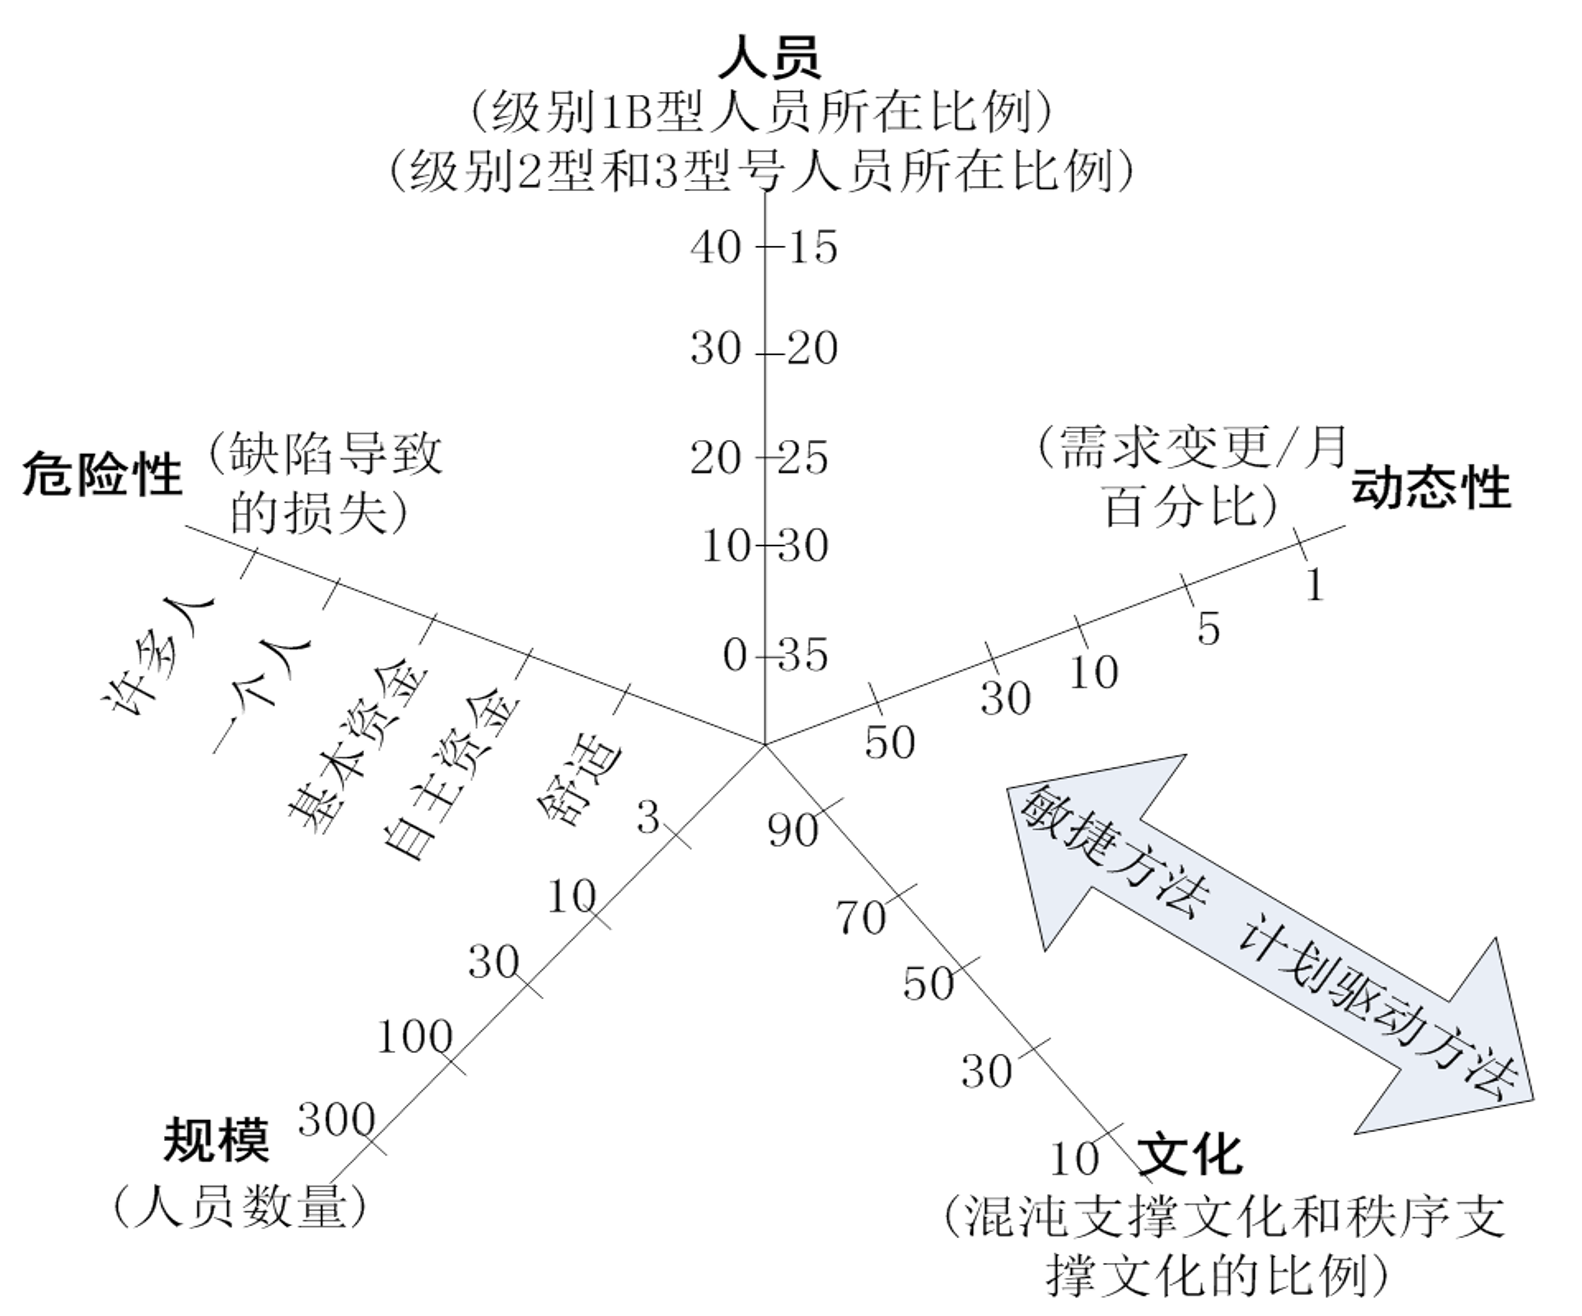
\includegraphics[width=0.55\textwidth]{images/基于风险分析平衡敏捷与规范.png}
    \vspace{-1em}
\end{figure}
\end{problem}

\subsection{PSP的质量管理}

\subsubsection{PSP质量观与质量策略}
软件项目的\textbf{日程、成本以及质量}三大目标统一于质量目标

什么是软件质量?
\begin{itemize}
    \item 与软件产品满足规定的和隐含的需求能力有关的特征或者特征的全体
    \item PSP中定义质量为满足用户需求的程度,需要明确用户需求的\textbf{范围}、\textbf{优先级}、\textbf{度量方式}
\end{itemize}

软件质量分为内外两部分的特性
\vspace{-0.8em}
\begin{multicols}{2}
    \begin{itemize}
        \item 其外部质量特性面向软件产品的最终用户
        \item 其内部质量特性不直接面向最终用户
    \end{itemize}
\end{multicols}
\vspace{-1em}

软件质量的不同视角
\begin{itemize}
    \item 软件质量为软件产品可以改变世界,使世界更加美好的程度。从用户的角度考察软件质量,用户满意度是最为重要的判断标准
    \item 软件质量是对人(用户)的价值,这一定义强调了质量的主观性,即对于同一款软件而言,不同的用户对其质量有不同的体验
\end{itemize}

\paragraph{面向用户的质量观}~{} \par
PSP中也采用了面向用户的质量观,定义质量为满足用户需求的程度。在这个定义中,就需要进一步明确:
\vspace{-0.8em}
\begin{multicols}{2}
    \begin{itemize}
        \item 用户究竟是谁?
        \item 用户需求的优先级是什么?
        \item 这种用户的优先级对软件产品的开发过程产生什么样的影响?
        \item 怎样来度量这种质量观下的质量水平?
    \end{itemize}
\end{multicols}
\vspace{-1em}

典型用户质量期望
\begin{itemize}
    \item 这款软件产品必须能够工作:因此可以使用缺陷管理代替质量管理
    \item 这款软件产品最好有较快的执行速度
    \item 这款软件产品最好在安全性、保密性、可用性、可靠性、兼容性、可维护性、可移植性等表现优异
\end{itemize}

指导意义
\vspace{-0.8em}
\begin{multicols}{2}
    \begin{itemize}
        \item 开发在前,运维在后
        \item \textbf{高质量开发确保DevOps中的价值顺畅流动}
        \item 个体软件工程师技能、过程直接影响产品质量
        \item PSP关注提升个体软件工程师工程技能
    \end{itemize}
\end{multicols}
\vspace{-1em}

\paragraph{质量策略}~{} \par
\vspace{-0.8em}
\begin{multicols}{2}
    \begin{itemize}
        \item 首先确保基本没有缺陷,然后再考察其他的质量目标
        \item 使用缺陷管理来代替质量管理
        \item 高质量的产品也就意味着组成软件产品的各个组件基本无缺陷
        \item 各个组件的高质量是通过高质量评审来实现的
    \end{itemize}
\end{multicols}
\vspace{-1em}

为什么有效?
\begin{itemize}
    \item 提高生产效率,通过关注每个组件的质量,往往可以避免在集成测试和系统测试消除
    \item 大量缺陷,减少消除代价,提升生产效率
\end{itemize}

\paragraph{质量路径 Quality Journey}~{} \par
为了追求极高的质量,你有哪些手段?
\vspace{-0.8em}
\begin{multicols}{2}
    \begin{enumerate}[label=\arabic*.]
        \item 各种测试
        \item 进入测试之前的产物质量提升
        \item 评审过程度量和稳定
        \item 质量意识和主人翁态度
        \item 个体 review 的度量和稳定
        \item 诉诸设计
        \item 缺陷预防
        \item 用户质量关——其他质量属性
    \end{enumerate}
\end{multicols}
\vspace{-1em}

\paragraph{考试题目}~{} \par
\begin{problem}
什么是面向用户的质量观?这对质量管理的策略有什么影响?
\end{problem}

\begin{problem}
请区分质量管理和缺陷管理之间的联系和差异,并解释为何在软件开发中将质量和生产效率两者进行妥协不合适?
\end{problem}

\begin{problem}
为了追求极高的软件产品的质量目标,可能有的方法和这些方法的先后顺序分别是什么?
\end{problem}

\begin{problem}
质量实践和质量管理是不一样的:质量实践包括测试等等,质量管理是对质量的管理,而不是实践,管理必须有上面所说的三个要素
\end{problem}

\subsubsection{发现缺陷的几个示例流程}

\paragraph{测试消除缺陷的典型流程}~{} \par
\vspace{-0.8em}
\begin{multicols}{2}
    \begin{enumerate}[label=\arabic*.]
        \item 发现待测程序的一个异常行为
        \item 理解程序的工作方式
        \item 调试程序,找到出错的位置,确定出错的原因:非常耗时,在项目后期可能会消耗数天甚至数周的时间
        \item 确定修改方案,修改缺陷
        \item 回归测试,以确认修改有效
    \end{enumerate}
\end{multicols}
\vspace{-1em}

\paragraph{评审发现缺陷的典型流程}~{} \par
在如下的步骤中,每一步消耗的时间都不会太多。尽管评审的技能因人而异,但是,通过适当培训和积累,有经验的评审者可以发现80\%左右的缺陷
\vspace{-0.8em}
\begin{multicols}{2}
    \begin{itemize}
        \item 遵循评审者的逻辑来理解程序流程
        \item 发现缺陷的同时,也知道了缺陷的位置和原因
        \item 修正缺陷
    \end{itemize}
\end{multicols}
\vspace{-1em}

\subsubsection{评审与测试}

\paragraph{评审检查表}~{} \par

\begin{figure}[H]
	\centering
	\vspace{-0.5em}	
	\subfloat{
	\begin{minipage}[c]{0.44\linewidth}
	\centering
	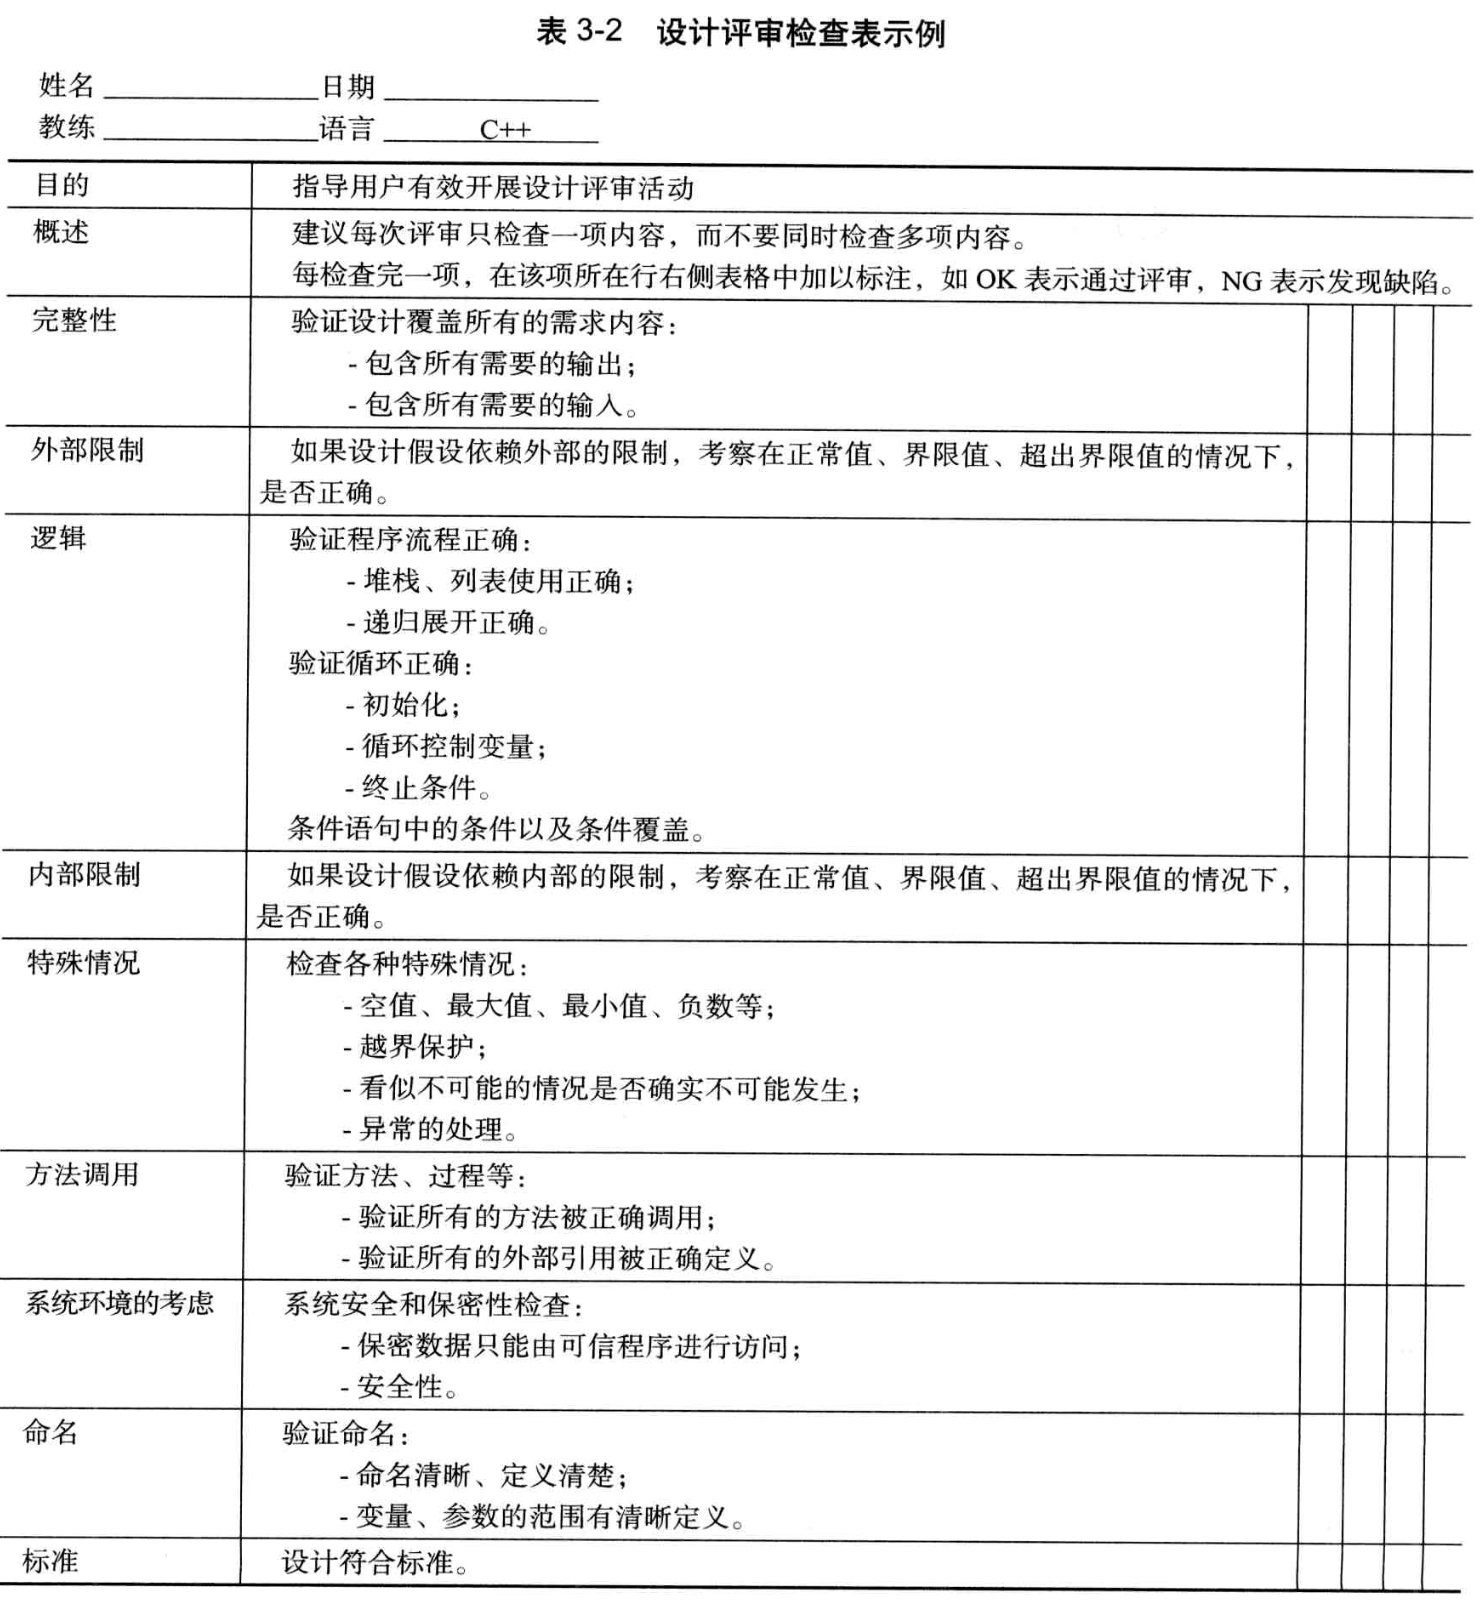
\includegraphics[width=\linewidth]{images/设计评审检查表示例.png}
	\end{minipage}
	}
    \hfill
	\subfloat{
	\begin{minipage}[c]{0.44\linewidth}
	\centering
	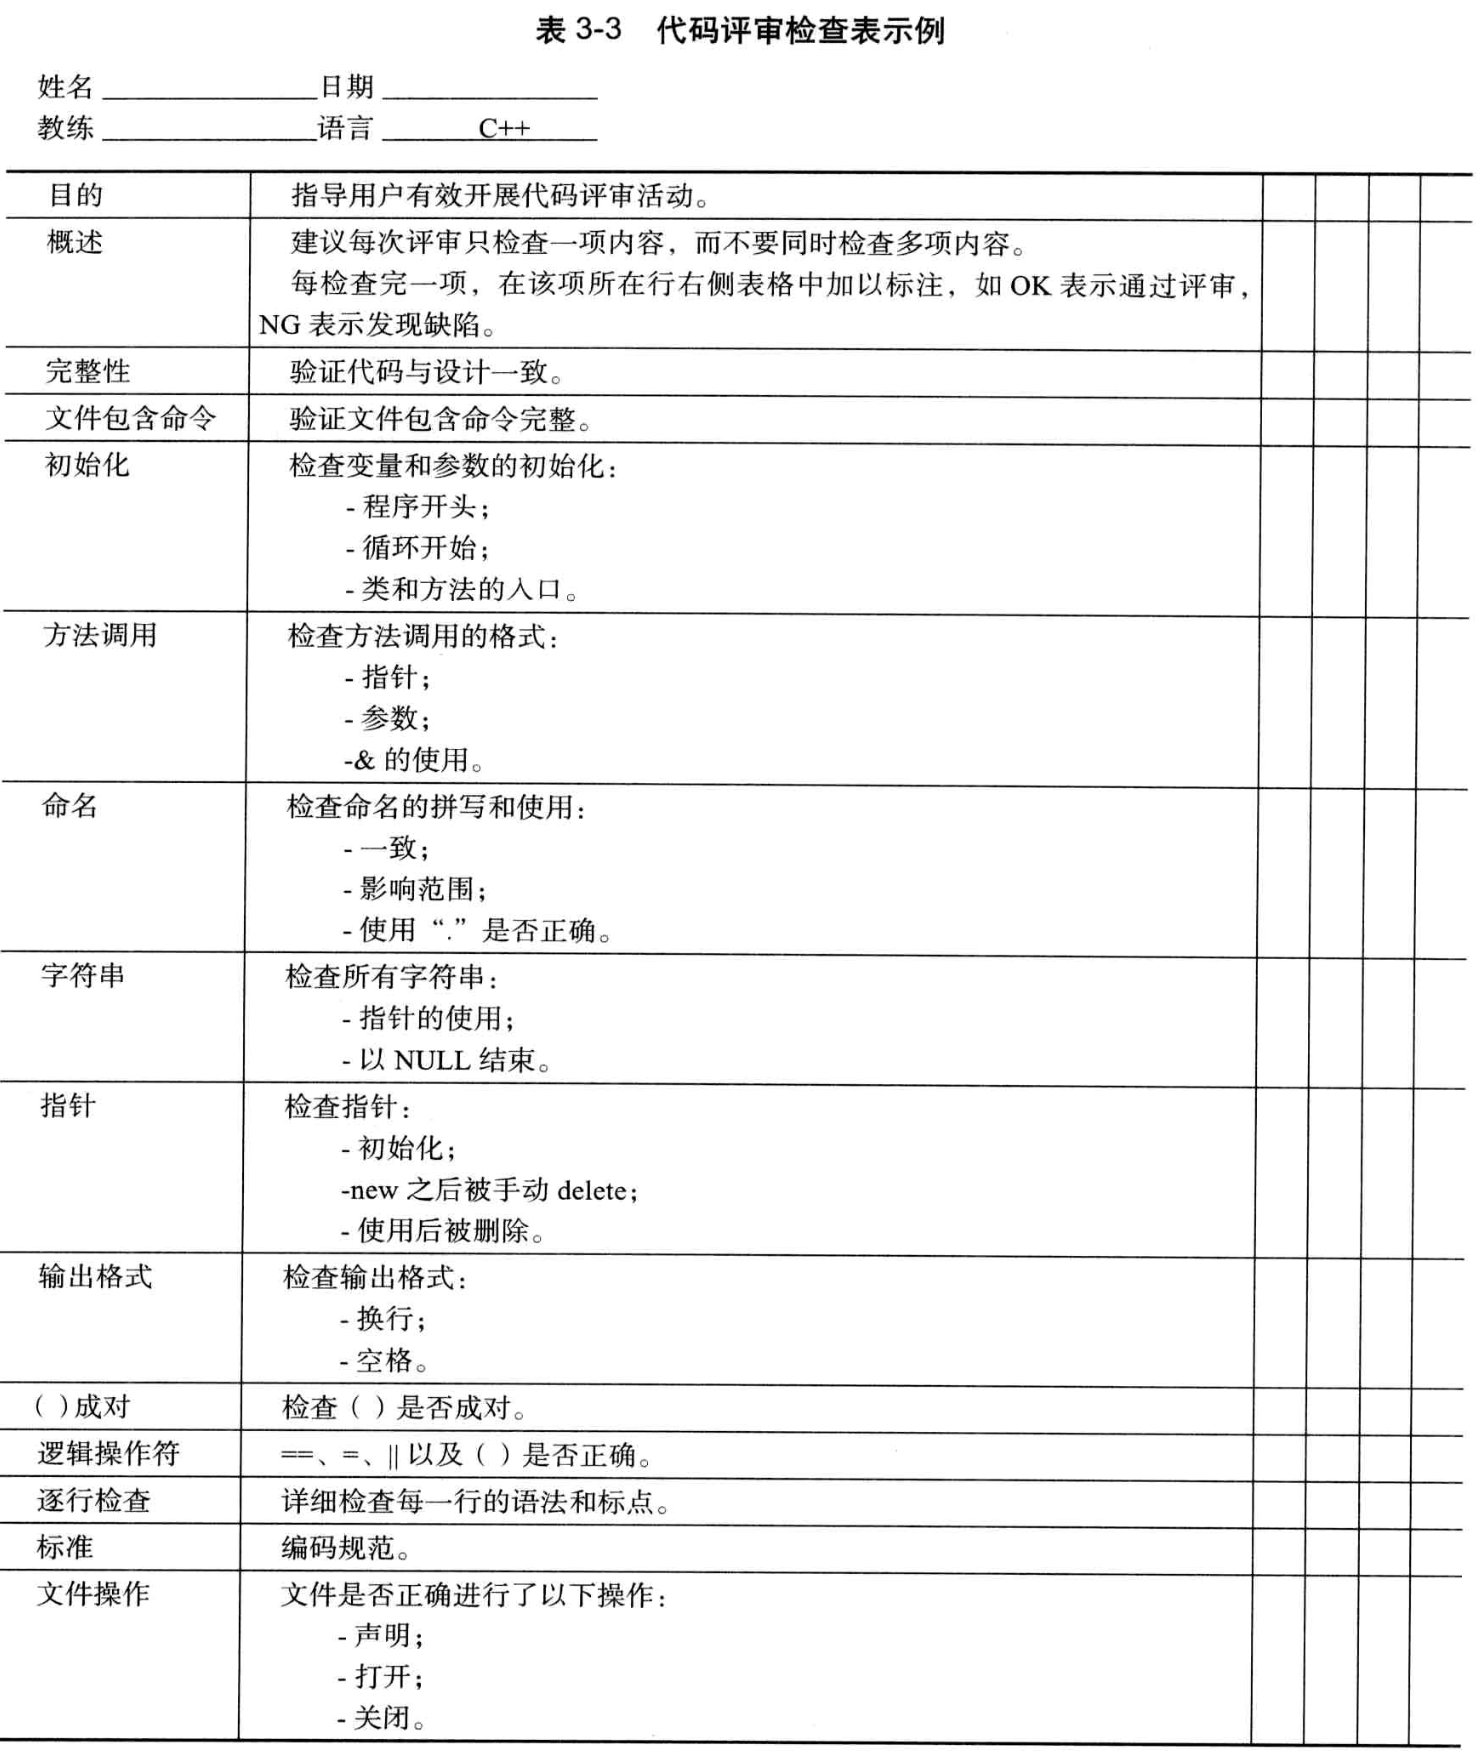
\includegraphics[width=\linewidth]{images/代码评审检查表示例.png}
	\end{minipage}
	}
	\centering
\end{figure}

\paragraph{评审形式}~{} \par
打印后评审效果更好
\begin{itemize}
    \item 单个屏幕可以展现的内容比较有限(评审对象比较复杂的时候,单个屏幕往往不能体现评审对象的整体结构、整体安全、整体性能以及其他整体属性)
    \item 评审人员的注意力:基于屏幕的评审往往容易受到干扰,从而影响评审人员的注意力
\end{itemize}

\paragraph{评审时机}~{} \par
编译、评审
\begin{itemize}
    \item 对于某些类型的缺陷而言,通过编译发现并消除的效率往往是通过评审发现并消除的数倍
    \begin{itemize}
        \item 越来越强大的编译器一般可以发现超过90\%的拼写错误
        \item 不管怎么努力,评审还有会遗漏约$20\sim 50$\%的语法错误
        \item 即便编译器遗漏了一些类似语法的错误,这些错误也不难通过单元测试消除
    \end{itemize}
\end{itemize}

评审、编译
\begin{itemize}
    \item 为了确保评审的效率,不管在评审之前有没有编译,评审的速度是一定的,也就意味着评审所需时间是一定的,那么如果先评审后编译,在编译阶段就可以节省较多的时间
    \item 编译器会大概会遗漏9\%左右的缺陷,从前面讨论可知,为了有较高的质量,这些缺陷仍然期望通过评审加以消除
    \item 有数据表明,编译过程中缺陷较多,往往意味着单元测试中缺陷也较多
    \item 即便单元测试也可以发现一些类似语法的错误,但是,毕竟还有些很难发现,而单元测试之后的一些缺陷消除环节的Pahse Yield往往还低于单元测试
    \item 编译之前评审也是一种自我学习的好机会
    \item 干净的编译,即编译过程没有缺陷对于软件工程师来说,也有极大的成就感
\end{itemize}

\paragraph{评审的具体形式}~{} \par
个人评审 $\rightarrow$ 小组评审

小组评审的意义
\begin{itemize}
    \item 有利于更好地发现缺陷,预防风险,提高Process Yield进而确保质量
    \item 在个人评审之后安排小组评审,也有利于提升个人的技能。特别是那些个人评审未发现而小组评审发现的缺陷,往往都需要引起足够的注意。软件工程师通过对这些缺陷的分析,往往可以学到很多东西
\end{itemize}

\paragraph{评审中缺陷预防过程中的缺陷数据选择}~{} \par
\begin{itemize}
    \item 选择那些在系统测试、验收测试以及应用环节出现的缺陷,特别是验收测试和应用环节中的缺陷,这些缺陷往往意味着软件开发过程本身有不足之处
    \item 选择那些在出现频率较高或者消除代价较高的缺陷,这些缺陷如果可以预防,往往可以节省较多开发的代价,从而体现缺陷预防的优势
    \item 选择那些预防方法容易识别和实现的缺陷,这样的策略容易让软件工程师迅速看到缺陷预防的好处,鉴定使用缺陷预防策略的信心
\end{itemize}

\subsubsection{PSP质量控制的衍生指标}

\paragraph{Yield指标}~{} \par
定义了各个阶段在消除缺陷方面的效率:Yield指标越高越好,Process Yield我们期望在80以上
$$Phase\ Yield = 100 \times \frac{\mbox{某个阶段发现的缺陷个数}}{\mbox{某个阶段注入的缺陷个数} + \mbox{进入该阶段前遗留的缺陷个数}}$$

$$Process\ Yield = 100 \times \frac{\mbox{第一次编译前发现的缺陷个数}}{\mbox{第一次编译前注入的缺陷个数}}$$

Yield可用于制定质量计划并且在项目执行阶段用于进行风险监控、预测、识别以及控制

\textbf{例:}计算Phase Yield。例如对于编码阶段来说,注入缺陷16个,消除缺陷 2 个,进入编码阶段遗留缺陷 4 个,那么该阶段的Phase Yield 就是10
\vspace{-0.5em}
\begin{table}[H]
    \centering
    \begin{tabular}{|c|c|c|c|c|}
    \hline
    \textbf{阶段名称} & \textbf{注入缺陷数} & \textbf{消除缺陷数} & \textbf{遗留缺陷数} & \textbf{Phase Yield}    \\ \hline
    设计            & 10             & 0              & 10             & 0                       \\ \hline
    设计评审          & 0              & 6              & 4              & $60=100 \times 6/ (0 + 10)$    \\ \hline
    编码            & 16             & 2              & 18             & $10=100 \times 2/(16 + 4)$     \\ \hline
    代码评审          & 0              & 9              & 9              & $50 = 100 \times 9 / (0 + 18)$ \\ \hline
    编译            & 0              & 5              & 4              & $55.6=100\times 5/(0+9)$       \\ \hline
    单元测试          & 1              & 5              & 0              & $100=100 \times 5 / (1 + 4)$   \\ \hline
    \end{tabular}
\end{table}
\vspace{-1em}

\textbf{例:}不使用历史数据的计算方法:
\begin{itemize}
    \item 在进行各个阶段Yield值的估算时,可以将单元测试阶段的Phase Yield设定为50
    \item 有资料表明,在测试中每发现一个缺陷,往往意味着还有一个缺陷没有被发现
    \item 那么也就意味着在上面的例子中,总共还有5个缺陷末被消除。将5个缺陷按照比例分配到各个缺陷的注入阶段,就可以重新计算Phase Yield的估算值
\end{itemize}

\vspace{-0.5em}
\begin{table}[H]
    \centering
    \begin{tabular}{|c|c|c|c|c|}
    \hline
    \textbf{阶段名称} & \textbf{注入缺陷数} & \textbf{消除缺陷数} & \textbf{遗留缺陷数} & \textbf{Phase Yield}    \\ \hline
    设计            & 11.85             & 0              & 11.85             & 0                       \\ \hline
    设计评审          & 0              & 6              & 5.85              & 50.6    \\ \hline
    编码            & 19             & 2              & 22.85             & 8     \\ \hline
    代码评审          & 0              & 9              & 13.85              & 41 \\ \hline
    编译            & 0              & 5              & 8.85              & 55.6     \\ \hline
    单元测试          & 1.15             & 5              & 5              & 50   \\ \hline
    \end{tabular}
\end{table}
\vspace{-1em}

Yield的计算是一种事后的质量控制手段,而且除非发现了所有的缺陷,否则很难非常精确地进行计算

\begin{problem}
基于Yield指标构建缺陷预测模型,并列举该模型的可能改进方案

总体思想:利用回归技术预测软件开发过程中各阶段的Inject Rate(缺陷注入率)和Yield(缺陷消除率)

Yield指标只能用来估算,不可以用来度量。结合Yield指标和下图,只需要知道如下指标就可以基于Yield指标构建一个基本的缺陷预测模型:
\vspace{-0.8em}
\begin{multicols}{2}
    \begin{itemize}
        \item 注入阶段注入多少缺陷
        \item 缺陷注入的密度(需求每一页注入多少缺陷)
        \item 缺陷注入的速度(每小时注入多少缺陷)
        \item 消除阶段的缺陷注入密度和速度。
        \item 历史数据中的软件规模、文档规模、开发人员规模
    \end{itemize}
\end{multicols}
\vspace{-1em}

步骤:
\vspace{-0.8em}
\begin{multicols}{2}
    \begin{enumerate}[label=\arabic*.]
        \item 确定纳入影响因子的数据以及数据度量方法
        \item 从系统历史库中收集历史数据,并进行整理
        \item 依照回归技术进行计算
        \item 在项目进行过程中不断收集数据,与预测数据进行比较,调整回归参数
        \item 项目过程中依据实际数据与预测数据的误差进行风险的预防、识别和控制
    \end{enumerate}
\end{multicols}
\vspace{-1em}

下图第一个消除步骤是需求评审,第二个消除步骤是设计评审,第三个消除步骤是测试评审

\begin{figure}[H]
    \vspace{-0.5em}
	\centering
	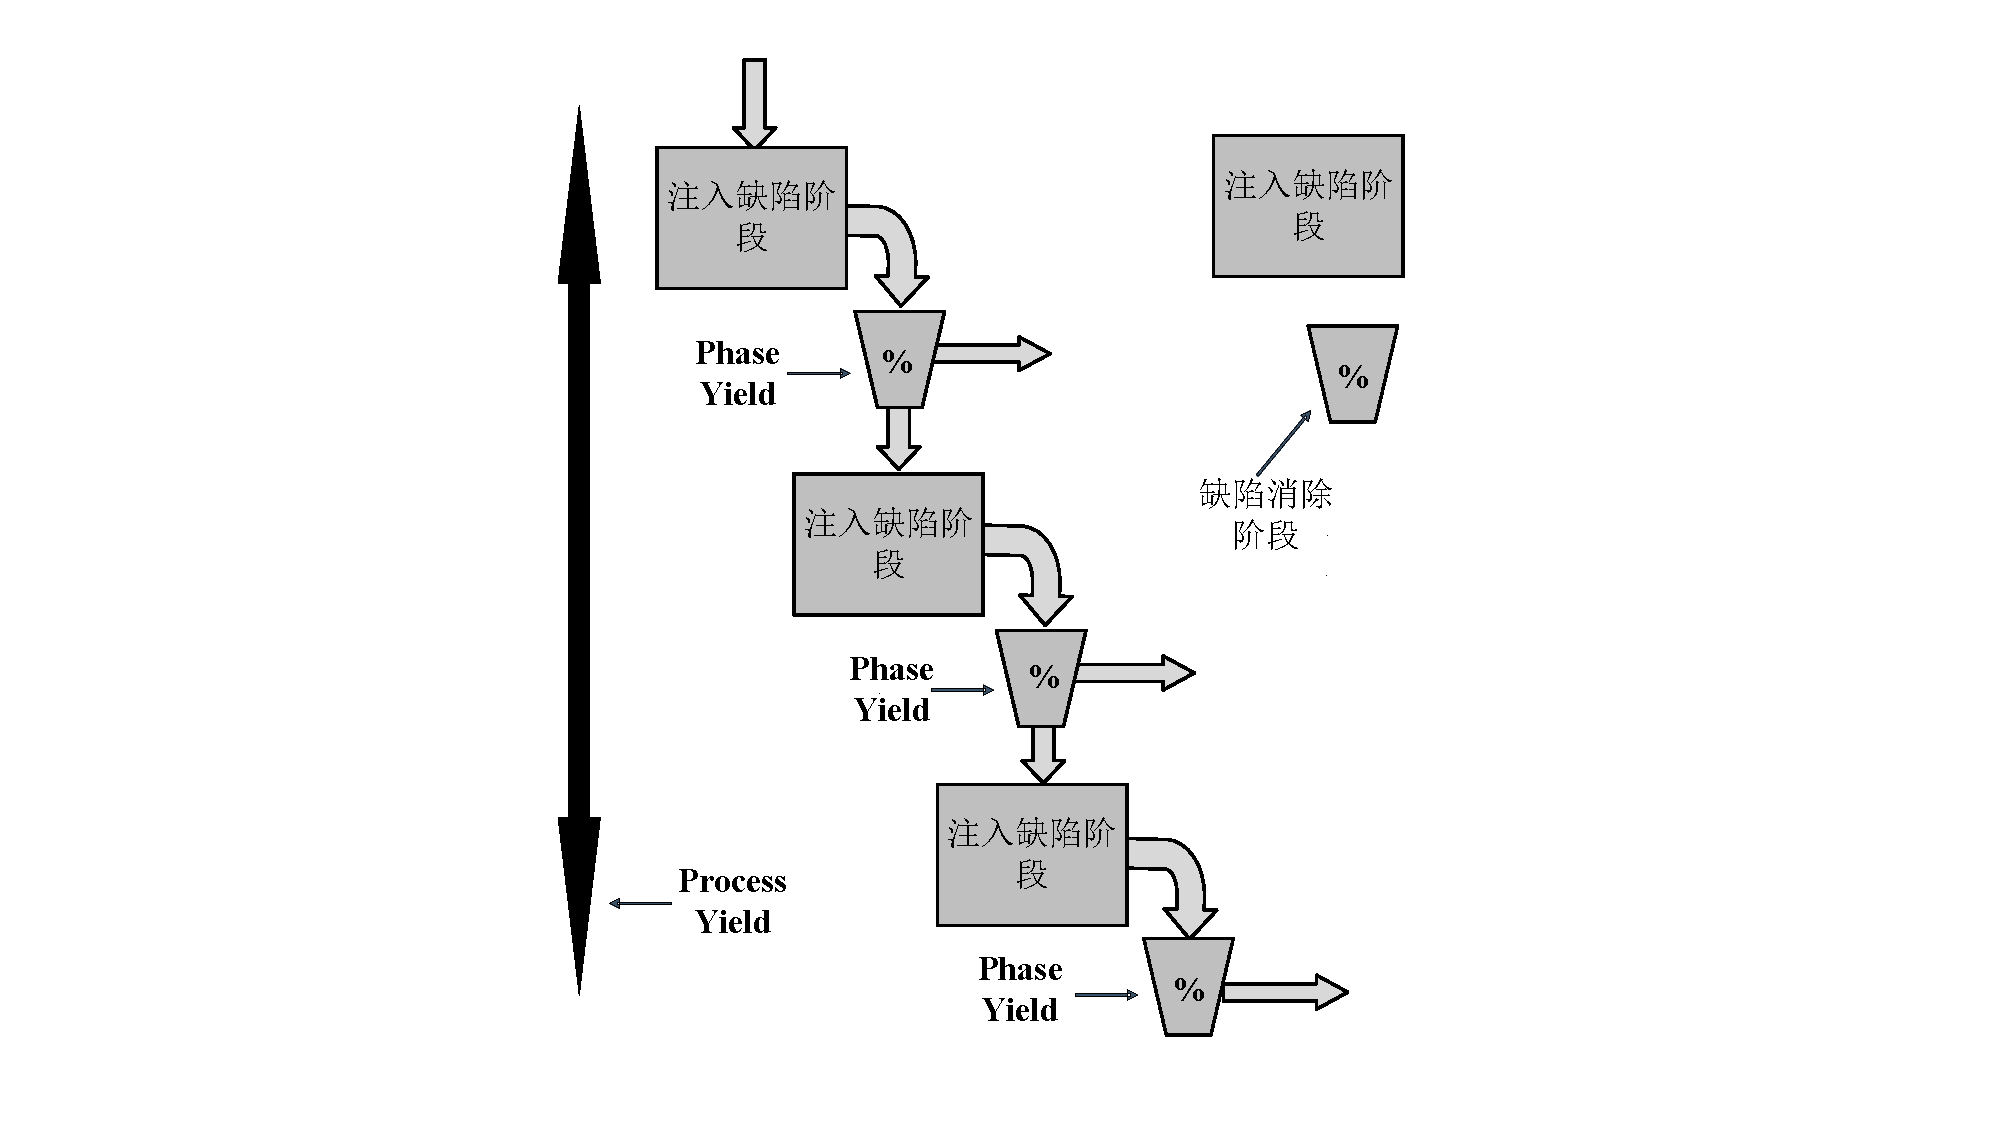
\includegraphics[width=0.42\textwidth]{images/缺陷在开发过程中注入和消除的示意图.pdf}
    \vspace{-1em}
\end{figure}

改进方案:
\begin{itemize}
    \item 结果受限于历史数据在简单性、可理解性、稳定性、可度量性、相关性等方法的质量。因此,维护历史数据。
    \item 影响因子的选择上面不仅仅需要有关软件规模的数据,还需要有关开发过程、开发文档、开发人员等方面的数据,并且需要将数据可度量化。
    \item 反馈模型。即在开发过程中随着实际数据的产生,将这些数据作为输入变量放入模型中以调整回归参数。
    \item (重要)可能的改进是假设注入水平和消除水平都符合正态分布,计算均值和标准差,因此,可以用蒙特卡罗方法模拟结果。
\end{itemize}
\end{problem}

\paragraph{A/FR}~{} \par
质量成本COQ(Cost of Quality)的三个重要组成部分为
\begin{itemize}
    \item 失效成本:分析失效现象、查找原因,做必要的修改所消耗的成本
    \item 质检成本:评价软件产品,确定其质量状况所消耗的成本
    \item 预防成本:识别缺陷根本原因、采取措施预防其再次发生所消耗的成本
\end{itemize}

A/FR (Appraisal toFailureRatio),质检失效比
\vspace{-0.8em}
\begin{multicols}{2}
    \begin{itemize}
        \item A/FR $=$ PSP质检成本 / PSP失效成本
        \item 质检成本 $=$ 设计评审时间 $+$ 代码评审时间
        \item 失效成本 $=$ 编译时间 $+$ 单元测试时间
    \end{itemize}
\end{multicols}
\vspace{-1em}

理论上,A/FR值越大,意味着质量越高,但A/FR值过大说明评审过多,则开发效率低下,因此PSP中A/FR期望值为2.0

\paragraph{PQI}~{} \par
PQI(Process Quality Index, 过程质量指标)为5个数据的乘积(以基准值作为1,最后结果越接近1,质量越高)
\begin{itemize}
    \item 设计质量:设计时间应该大于编码时间,$\min(\frac{\scriptsize{\mbox{设计时间}}}{\scriptsize{\mbox{编码时间}}}, 1)$
    \item 设计评审质量:设计评审的时间应该大于设计时间的50\%,$\min(2 \times \frac{\scriptsize{\mbox{设计评审时间}}}{\scriptsize{\mbox{设计时间}}}, 1)$
    \item 代码评审质量:代码评审时间应该大于编码时间的50\%,$\min(2 \times \frac{\scriptsize{\mbox{代码评审时间}}}{\scriptsize{\mbox{编码时间}}}, 1)$
    \item 代码质量:代码的编译缺陷密度应当小于10个/千行,$\min(\frac{20}{\scriptsize{\mbox{编译缺陷密度}} + 10}, 1)$
    \item 程序质量:代码的单元测试缺陷密度应当小于5个/千行,$\min(\frac{10}{\scriptsize{\mbox{单元测试缺陷密度}} + 5}, 1)$
\end{itemize}

用途:
\vspace{-0.8em}
\begin{multicols}{3}
    \begin{itemize}
        \item 判断模块开发质量
        \item 规划质量活动计划
        \item 过程改进
    \end{itemize}
\end{multicols}
\vspace{-1em}

\begin{problem}
解释PQI指标,如何计算,如何使用
\end{problem}

\paragraph{Review Rate}~{} \par
评审的速度(Review Rate)是一个用以指导软件工程师开展有效评审的指标,高质量的评审需要软件工程师投入足够的时间进行评审
\begin{itemize}
    \item 在PSP的实践中,代码评审速度小于200 LOC/小时,文档评审速度小于4 Page/小时
\end{itemize}

\paragraph{DRL}~{} \par
\begin{wraptable}{r}{7cm}
    \centering
    \vspace{-1.5em}
    \begin{tabular}{|c|c|c|}
        \hline
        \textbf{阶段} & \textbf{缺陷个数/小时} & \textbf{DRL (UT)} \\ \hline
        设计评审        & 3.6              & 1.03              \\ \hline
        编码评审        & 8                & 2.29              \\ \hline
        单元测试        & 3.5              & 1                 \\ \hline
        \end{tabular}
    \vspace{-1.5em}
\end{wraptable}
缺陷消除效率比(DRL, Defect-Removal-Leverage)度量的是不同缺陷消除手段消除缺陷的效率

计算方法:以某个测试阶段(一般为单元测试)每小时发现的缺陷数为基础,其他阶段每小时发现缺陷数与该测试阶段每小时发现的缺陷的比值就是DRL

\paragraph{考试题目}~{} \par
\begin{problem}
请解释A/FR,PQI的计算方式,并且解释这两个指标有什么用途?
\end{problem}

\begin{problem}
请结合A/FR、PQI、Review Rate、DRL、Yield尽可能具体描述一个软件项目应该如何从多方面来确保开发的高质量?

这些指标既是开发过程中质量管理的一些参考指标,同时也体现在计划安排中应该注意的质量元素。具体如下:
\begin{itemize}
    \item 在项目计划过程中应该安排确保高质量开发结果的活动,例如,按照A/FR、PQI等指标的要求,安排对各类产物(文档和代码)的个人评审和小组评审
    \item 这些评审活动应该满足一定的要求,特别体现在时间方面。例如,评审时间应该多于测试时间的两倍以上(A/FR);评审时间应该是相应开放时间的50\%以上(PQI);评审速度要求(Review Rate)等
    \item 充分借鉴质量指标所体现的开发质量状况,尽早制订相应的质量补救措施。例如,PQI所体现的缺陷密度、所有上述指标的参考值等等。一旦超标,往往意味着质量方面有偏差,应当及时补救
    \item 利用Yield等指标,构建质量预测模型,更加积极(Proactive)地判定和控制开发质量
    \item 依据PQI和Yield指标所体现的信息,通过过程改进来提升开发质量
\end{itemize}
\end{problem}

\subsubsection{考试题目}
\begin{problem}
如果对质量的追求是无止境的,在不考虑资源和成本的前提下,有哪些可能有效的策略?
\vspace{-0.8em}
\begin{multicols}{2}
    \begin{enumerate}[label=\arabic*.]
        \item 重视测试,并且将测试过程文档化并且稳定化
        \item 重视小组评审,同样定义评审过程,并且使得评审过程的performance稳定化
        \item 重视个人评审,提升评审者技能
        \item 重视设计
        \item 开展设计验证
        \item 质量策略:参考上面
    \end{enumerate}
\end{multicols}
\vspace{-1em}
\end{problem}

\subsection{PSP的设计}
PSP设计过程的关注点并不是具体的设计方法,而是设计的步骤定义以及设计的表现形式

\subsubsection{设计与质量的关系}
\vspace{-0.8em}
\begin{multicols}{2}
    \begin{itemize}
        \item 低劣的设计是导致在软件开发中返工、不易维护以及用户不满的主要原因
        \item 充分设计可以显著减少最终程序的规模,提升质量
        \item 设计本身也是一种排除错误的过程
    \end{itemize}    
\end{multicols}
\vspace{-1em}

\subsubsection{设计的过程}
\begin{figure}[H]
    \vspace{-0.5em}
	\centering
	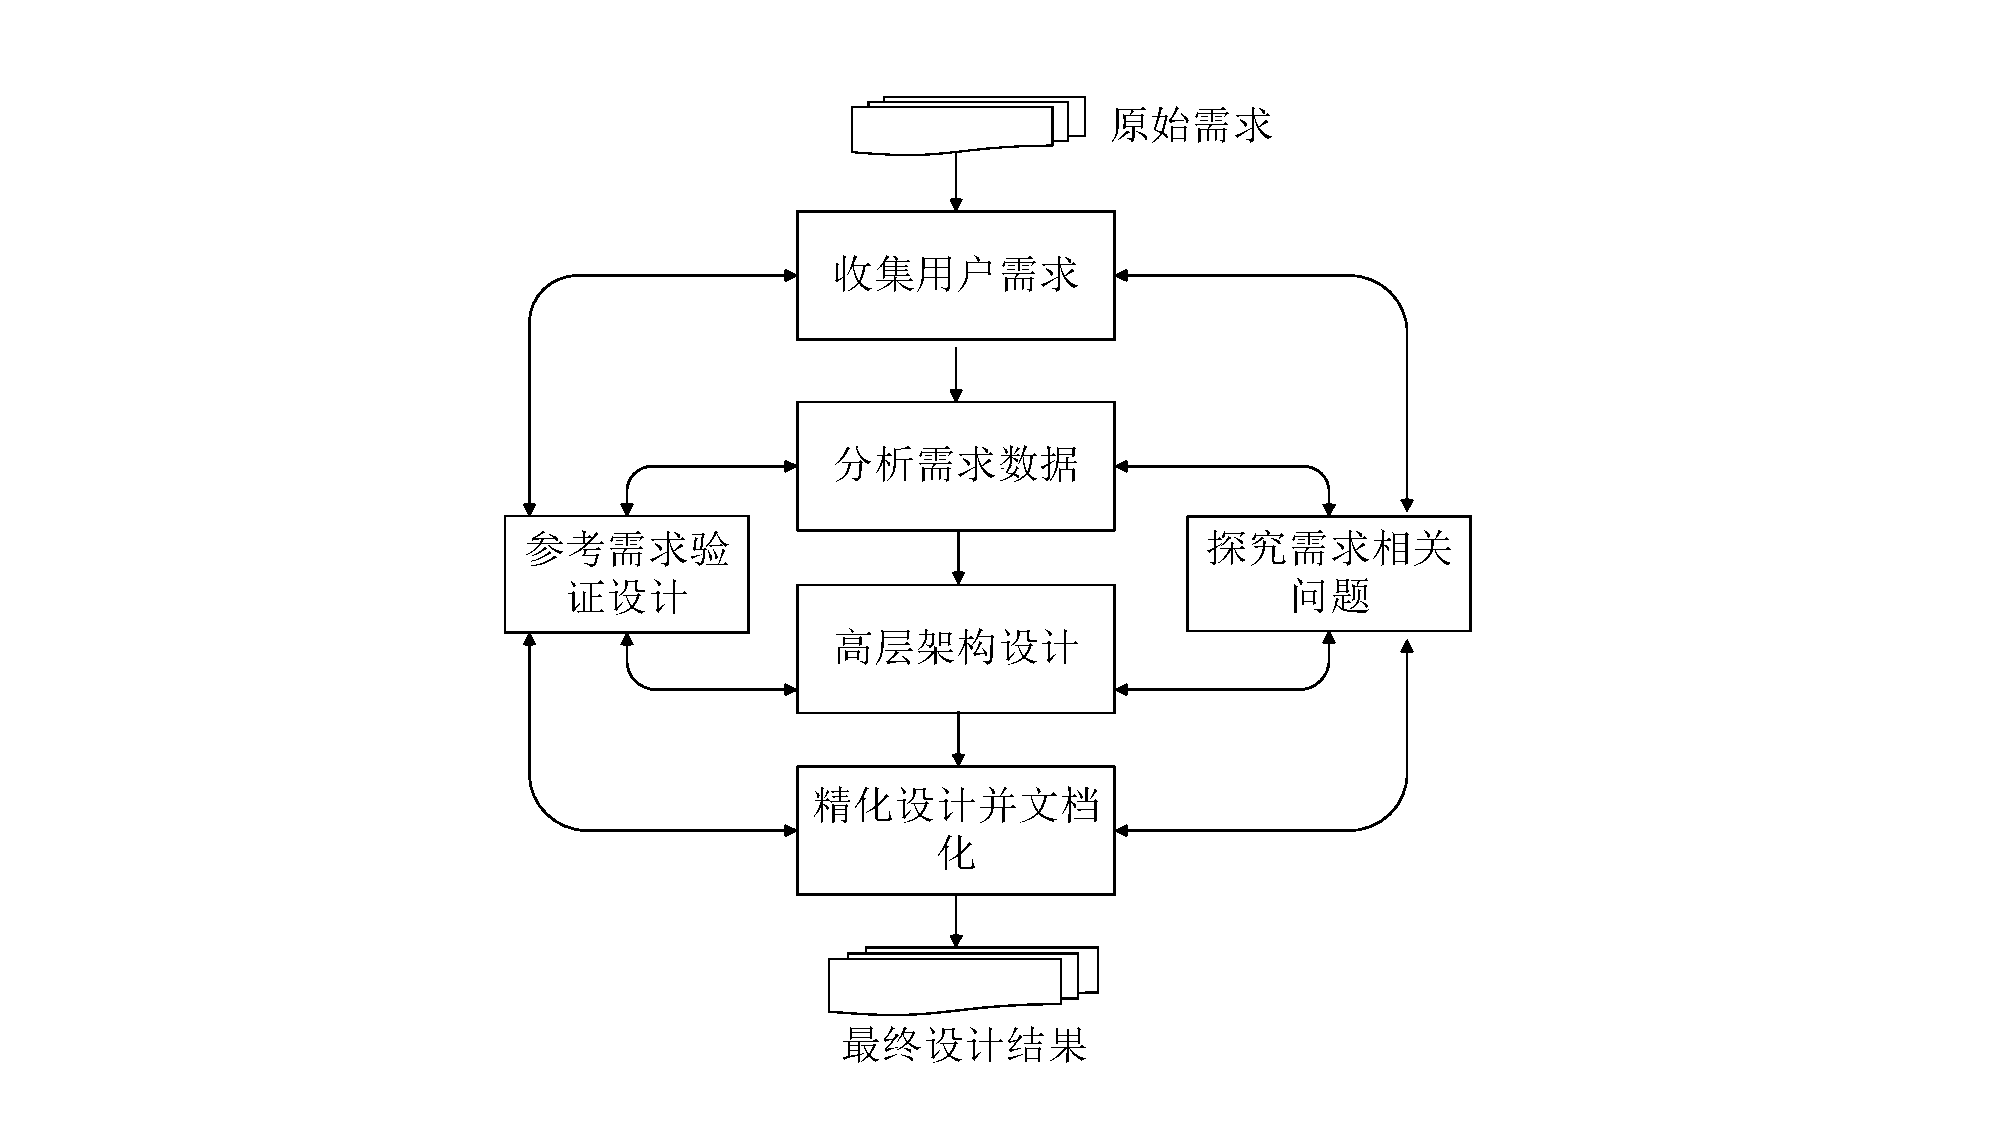
\includegraphics[width=0.5\textwidth]{images/PSP设计过程.pdf}
    \vspace{-1em}
\end{figure}

\subsubsection{设计什么?}
\vspace{-0.8em}
\begin{multicols}{2}
    \begin{enumerate}[label=\arabic*.]
        \item 设计目标程序在整个应用系统中的位置
        \item 设计目标程序的使用方式
        \item 设计目标程序与其他组件以及模块之间的关系
        \item 设计目标程序外部可见的变量和方法
        \item 设计目标程序内部运作机制
        \item 设计目标程序内部静态逻辑
    \end{enumerate}
\end{multicols}
\vspace{-1em}

\subsubsection{设计内容}
\vspace{-0.5em}
\begin{table}[H]
    \centering
    \begin{tabular}{|c|c|c|}
    \hline
                  & \textbf{动态信息} & \textbf{静态信息}  \\ \hline
    \textbf{外部信息} & 交互信息(服务、消息等)  & 功能(继承、类结构等)    \\ \hline
    \textbf{内部信息} & 行为信息(状态机)     & 结构信息(属性、业务逻辑等) \\ \hline
    \end{tabular}
\end{table}
\vspace{-1em}

\subsubsection{设计模板}
\begin{wraptable}{r}{6cm}
    \centering
    \vspace{-1em}
    \resizebox{6cm}{!}{\begin{tabular}{|c|c|c|}
        \hline
                      & \textbf{动态信息} & \textbf{静态信息} \\ \hline
        \textbf{外部信息} & OST/FST       & FST           \\ \hline
        \textbf{内部信息} & SST           & LST           \\ \hline
    \end{tabular}}
    \caption*{PSP设计模板展现的信息}
    \vspace{-1.5em}
\end{wraptable}
PSP设计模板
\begin{itemize}
    \item 操作规格模板(Operational Specification Template, OST)
    \item 功能规格模板(Functional Specification Template, FST)
    \item 状态规格模板(State Specification Template, SST)
    \item 逻辑规格模板(Logical Specification Template, LST)
\end{itemize}


\paragraph{操作规格模板OST}~{} \par
\begin{itemize}
    \item 描述系统与外界的交互,用于场景描述:也就是用户与待设计系统的正常情况和异常情况下的交互
    \item 定义测试场景和测试用例,用来与用户讨论需求的基础,特别是操作相关的需求描述
    \item 与UML比较:用例图、时序图
\end{itemize}

\paragraph{功能规格模板FST}~{} \par
\vspace{-0.8em}
\begin{multicols}{2}
    \begin{itemize}
        \item 描述系统的对外接口,是一种静态信息的展现
        \item 提供的典型信息有类和继承关系、外部可见的属性和方法等
        \item 用形式化符号等方法描述方法等行为,消除二义性
        \item 与UML对比:UML类图,但类图的方法的行为没有描述
    \end{itemize}
\end{multicols}
\vspace{-1em}

\paragraph{状态规格模板SST}~{} \par
可以精确定义程序的所有状态、状态之间的转换以及伴随着每次状态转换的动作

SST模板中,需要描述如下的信息
\vspace{-0.8em}
\begin{multicols}{3}
    \begin{itemize}
        \item 所有状态的名称
        \item 所有状态的简要描述
        \item 在 SST 中需要使用的参数和方法的名称与描述
        \item 状态转换的条件
        \item 状态转换是发生的动作
    \end{itemize}
\end{multicols}
\vspace{-1em}

与UML对比:UML状态图

\paragraph{逻辑规格模板LST}~{} \par
可以精确描述系统的内部静态逻辑。为了消除描述的二义性,一般建议使用伪代码配合形式化符号来描述设计结果

LST模板中,需要描述如下的信息
\vspace{-0.8em}
\begin{multicols}{2}
    \begin{itemize}
        \item 关键方法的静态逻辑
        \item 方法的调用
        \item 外部引用
        \item 关键数据的类型和定义
    \end{itemize}
\end{multicols}
\vspace{-1em}

与UML对比:没有对应图

\paragraph{UML}~{} \par
\begin{itemize}
    \item UML图有用例图、时序图、类图、状态机图
    \item UML的用例图和时序图提供了与PSP中OST同样的信息
    \item UML中的时序图和类图所描述的类之间的关系以及对象之间的交互信息在PSP的4个设计模板中没有对应的内容
    \item UML类图中记录了方法的型构,然而方法的行为没有描述,这一点在PSP的FST中有相应的内容
    \item PSP中的LST用以描述程序的静态逻辑,这在UML没有对应的图示方法
    \item UML中的状态图与SST描述的状态图类似,但是SST中描述的关于状态、状态转换条件以及状态转换中的动作没有对应的UML图示方法
\end{itemize}

\paragraph{考试题目}~{} \par
\begin{problem}
请解释设计的层次的概念和意义,并解释如何将PSP的4个设计模版应用在不同的设计层次之中?
\begin{figure}[H]
    \vspace{-0.5em}
	\centering
	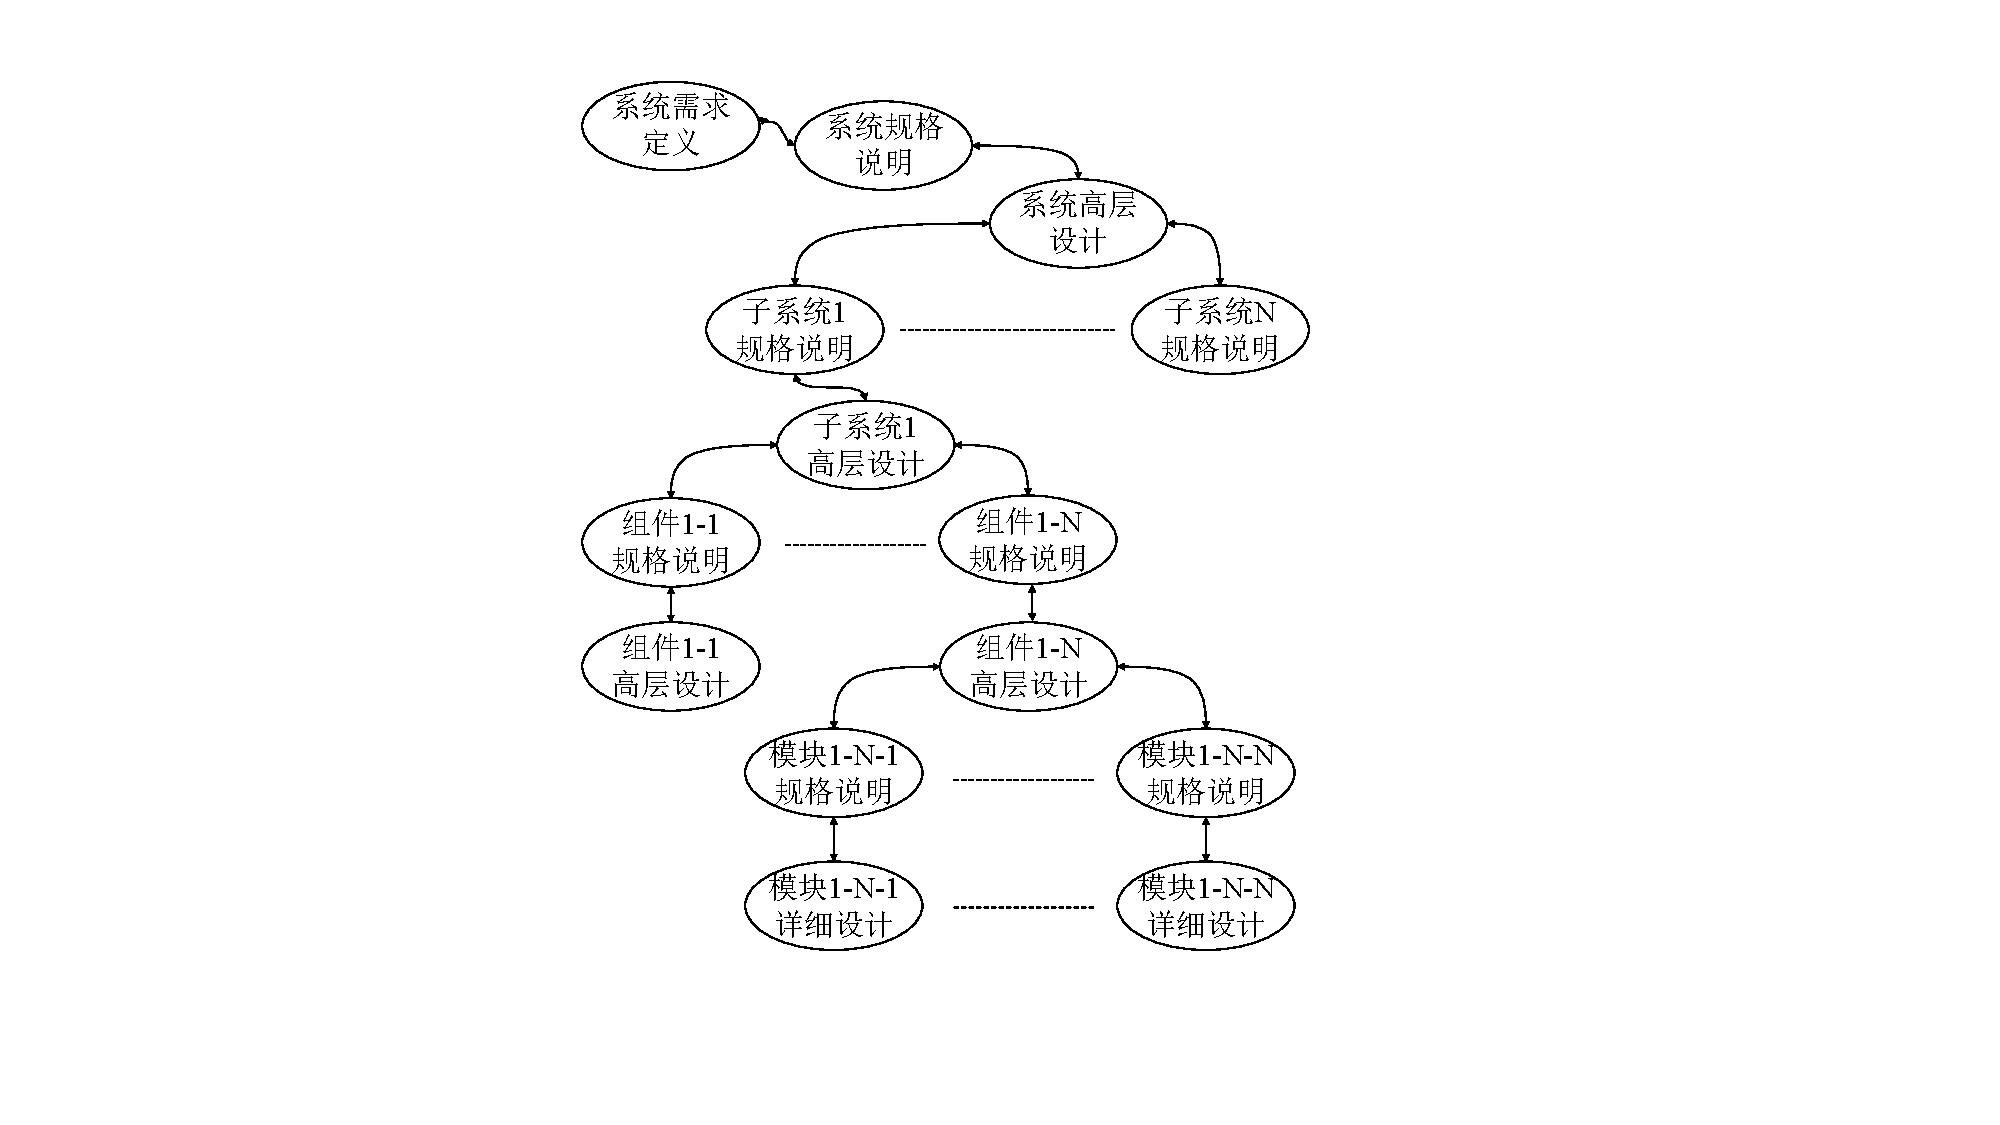
\includegraphics[width=0.47\textwidth]{images/设计的层次.pdf}
    \vspace{-1em}
\end{figure}
\end{problem}

\subsubsection{PSP设计验证方法}
意义:简单评审不足以发现复杂缺陷

\paragraph{状态机验证}~{} \par
检查状态机的完整性和正交性
\begin{itemize}
    \item 完整性:对于状态机中任何一个状态,对应的所有条件组合,下一个状态的转换都有定义
    \item 正交性:对于状态机中任何一个状态,其所有下一个状态的转换条件都不能相同
\end{itemize}

验证步骤:
\vspace{-0.8em}
\begin{multicols}{2}
    \begin{enumerate}[label=\arabic*.]
        \item 检查状态机,消除死循环和陷阱状态
        \item 检查状态转换,验证完整性和正交性
        \item 评价状态机,检验是否体现设计意图
    \end{enumerate}
\end{multicols}
\vspace{-1em}

示例:使用状态图,检查死循环和陷阱状态;使用真值表来进行分析
\begin{figure}[H]
    \vspace{-0.5em}
	\centering
	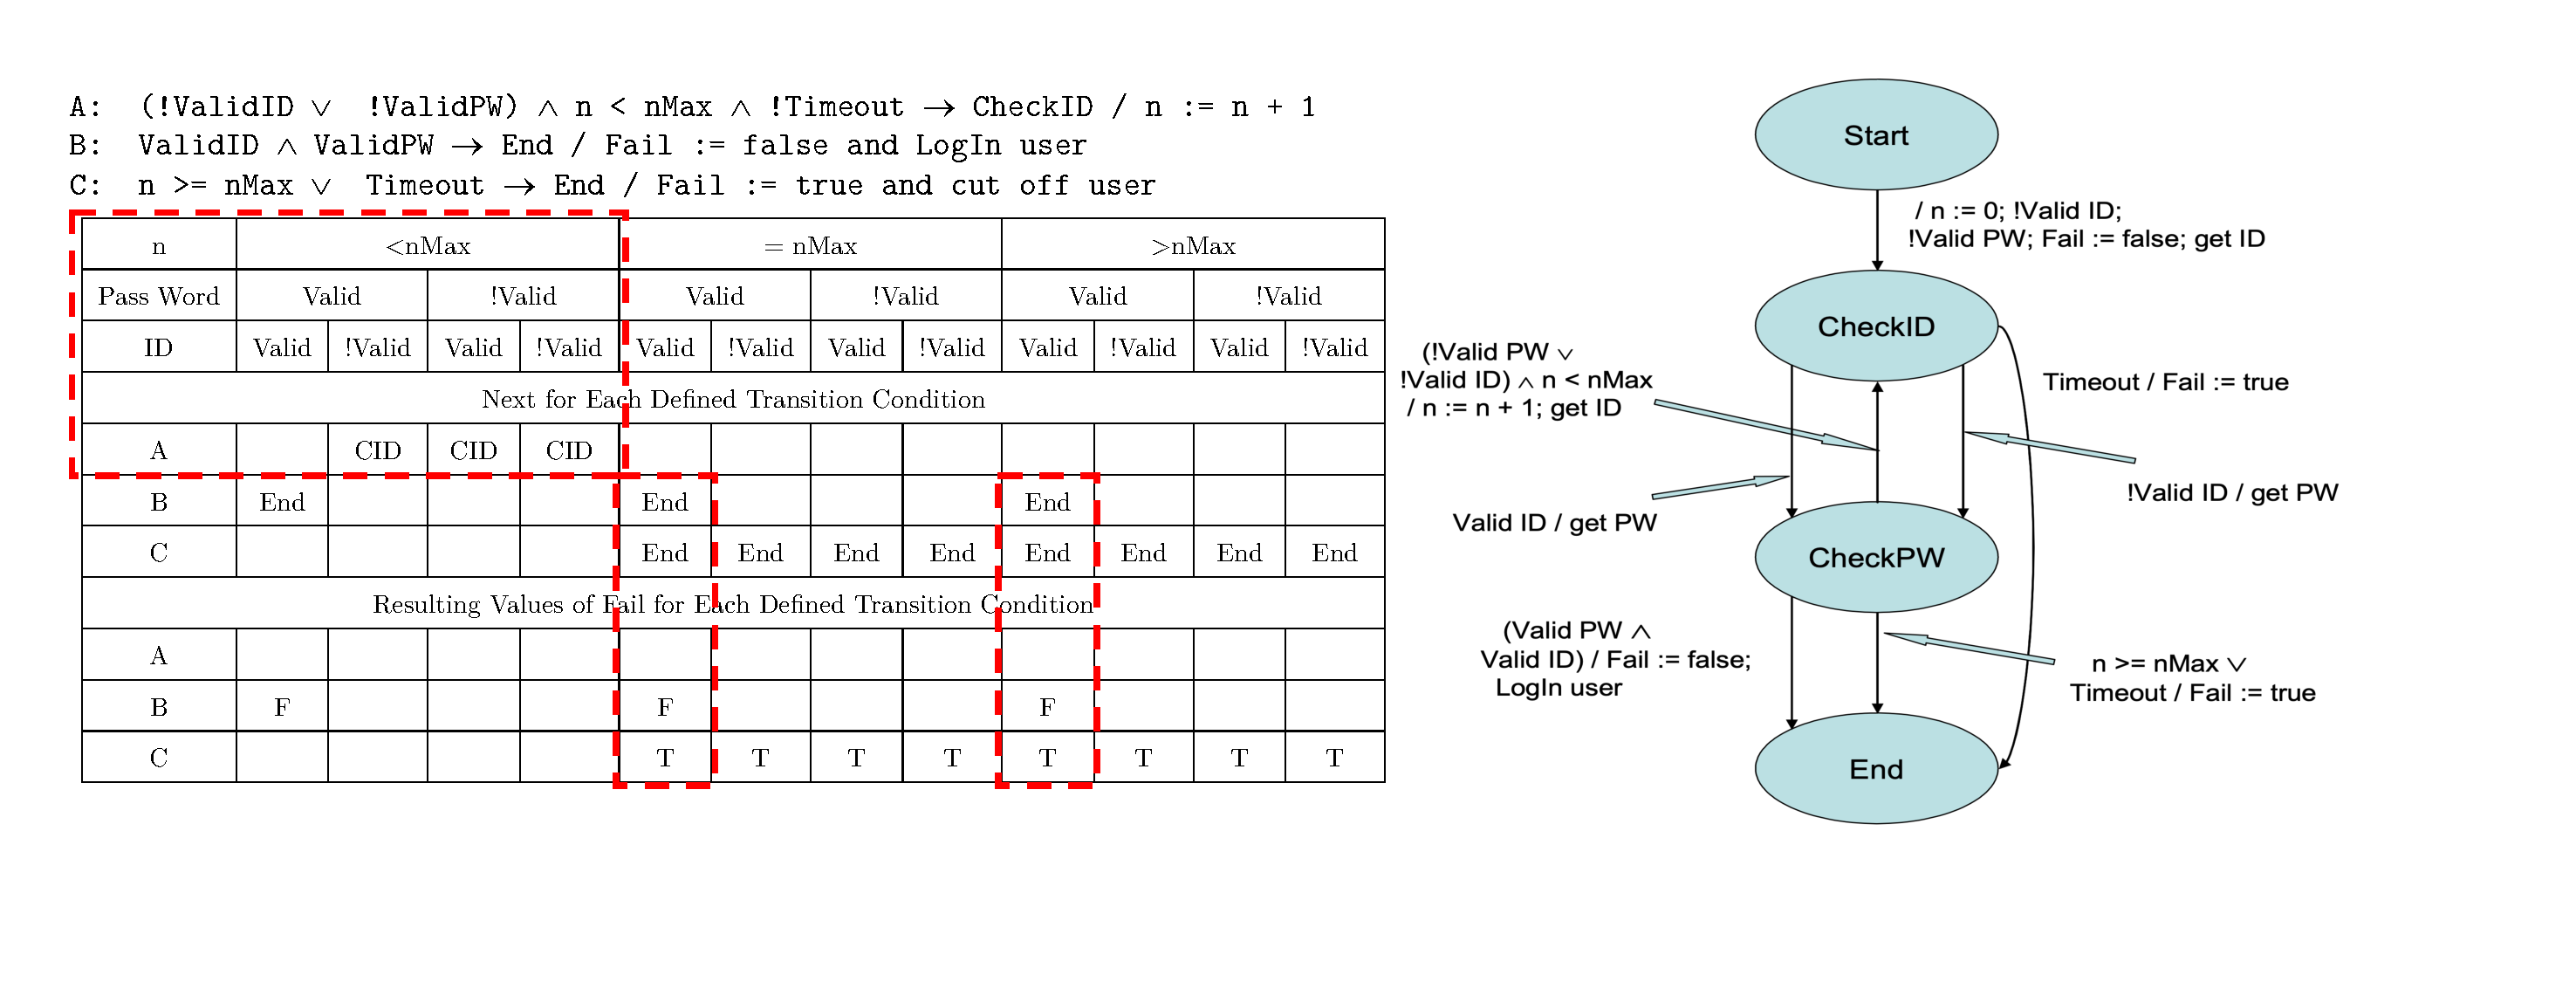
\includegraphics[width=\textwidth]{images/状态机示例.pdf}
    \vspace{-3em}
\end{figure}

\paragraph{符号化验证}~{} \par
将描述设计的逻辑规格(一般用伪代码程序表示)用代数符号来表示,然后系统地开展分析和验证

验证步骤:
\vspace{-0.8em}
\begin{multicols}{2}
    \begin{enumerate}[label=\arabic*.]
        \item 识别伪码程序中的关键变量
        \item 将这些变量使用代数符号表示,重写伪码程序
        \item 分析伪码程序的行为
    \end{enumerate}
\end{multicols}
\vspace{-1em}

示例:交换两个变量的值
\begin{figure}[H]
    \vspace{-0.5em}
	\centering
	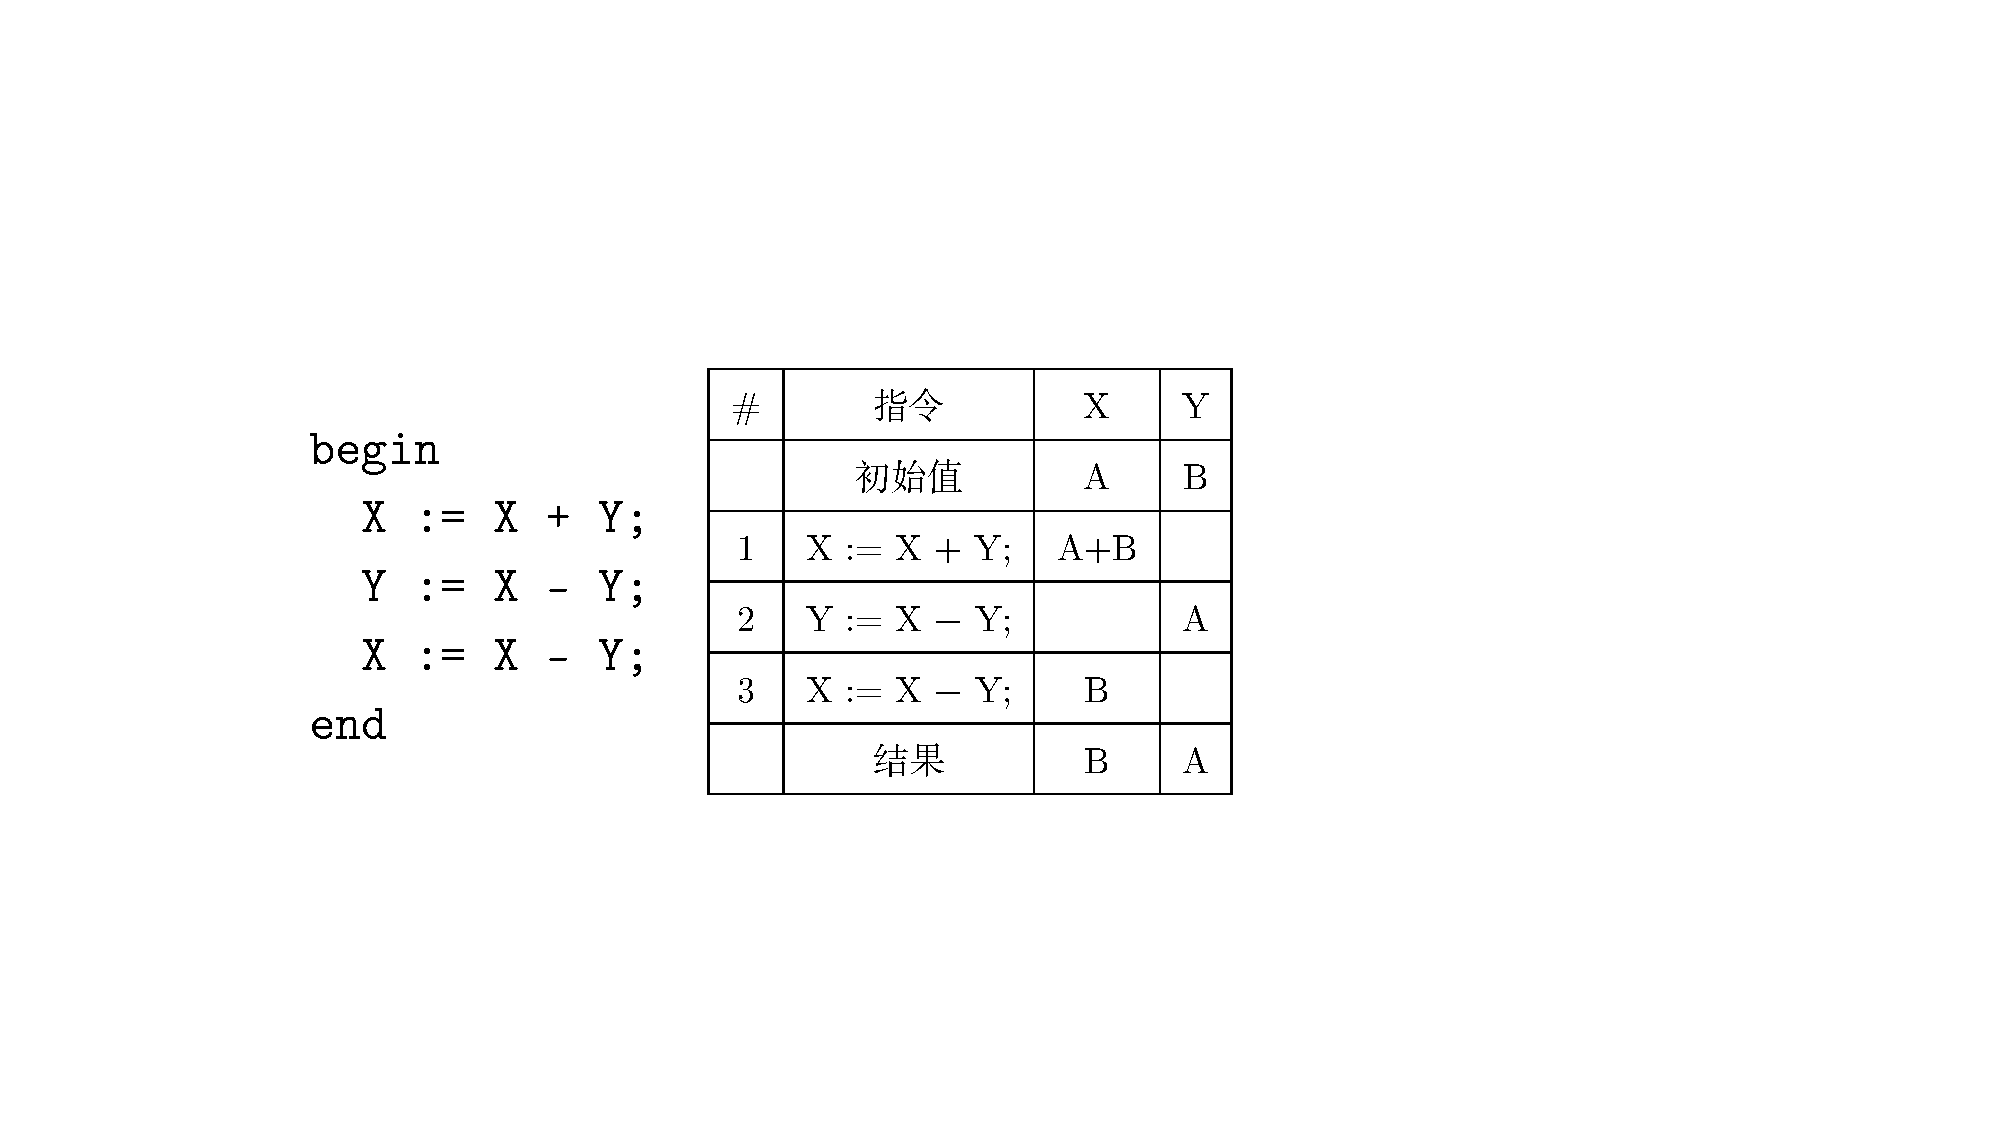
\includegraphics[width=0.5\textwidth]{images/符号化执行验证示例.pdf}
    \vspace{-1em}
\end{figure}

\vspace{-0.5em}
\begin{spacing}{1.2}
    \centering
    \begin{longtable}{|m{7.2cm}|m{7.2cm}|}
        \hline
        \multicolumn{1}{|c|}{\textbf{优点}} & \multicolumn{1}{c|}{\textbf{缺点}} \\ \hline
        \vspace{-1em}
        \begin{enumerate}[label=\arabic*.,leftmargin=1em]
            \item 实施简单,可以给出一般化的验证结果
            \item 适用于不复杂的算法,特别是遗漏系统的改造中,应用这种方法识别和理解原有的设计
            \vspace{-1.3em}
        \end{enumerate}
        & 不适合于有复杂逻辑的场合;纯手工验证方法容易引入错误
        \\ \hline
    \end{longtable}
	\end{spacing}
\vspace{-1em}

\paragraph{执行表验证}~{} \par
步骤:
\vspace{-0.8em}
\begin{multicols}{2}
    \begin{enumerate}[label=\arabic*.]
        \item 识别伪码程序的关键变量
        \item 构建表格,表格左侧填入主要程序步骤,右侧填入关键变量
        \item 初始化被选定的变量
        \item 跟踪被选择的关键变量的变化情况,从而判断程序行为
    \end{enumerate}
\end{multicols}
\vspace{-1em}

优点:实施简单;结果可靠,可用于复杂逻辑的验证

缺点:每次只能验证一个用例;手工验证比较耗时,容易引入错误

\paragraph{跟踪表验证}~{} \par
步骤:
\vspace{-0.8em}
\begin{multicols}{2}
    \begin{enumerate}[label=\arabic*.]
        \item 识别伪码程序的关键变量
        \item 构建表格,表格左侧填入主要程序步骤,右侧填入关键变量
        \item 初始化被选定的变量
        \item 识别将伪码程序符号化的机会,并加以符号化
        \item 定义并且优化用例组合
        \item 跟踪被选择的关键变量的变化情况,从而判断程序行动
    \end{enumerate}
\end{multicols}
\vspace{-1em}

跟踪表应用符号化以及用例识别等方法,对程序的一般化行为进行验证,是执行表验证的补充,可以每次验证多个用例,从而提供更加高效地开展验证工作

\paragraph{正确性验证}~{} \par
将伪码程序当做数字定理,采用形式化方法加以推理和验证

步骤:
\vspace{-0.8em}
\begin{multicols}{2}
    \begin{enumerate}[label=\arabic*.]
        \item 分析和识别用例
        \item 对于复杂伪码程序的结构,应用正确性验证的标准问题逐项加以验证
        \item 对于不能明确判断的复杂程序结果,使用跟踪表等辅助验证
    \end{enumerate}
\end{multicols}
\vspace{-1em}

While-Do循环的验证
\begin{enumerate}[label=\arabic*.]
    \item 条件1:condition 是否最终一定会为“假”,从而使得循环可以结束。
    \item 条件2:condition 为“真”的时候,单独的循环结构执行结果与循环体再加一个循环结构,其执行结果是否一致?
    \item 条件3:condition 为“假”的时候,循环体内所有变量是否未被修改?
\end{enumerate}
